\chapter{Convolutional Neural Network for predicting morphometry landmarks}
In the previous chapter, we have studied two CNNs \cite{sun2013deep, cintas2016automatic} that applied to predict the keypoints on human face and human ear. Then, we have applied their methods to detect the landmarks (keypoints) on thorax of beetle but the obtained results are not really impressed. In this chapter, based on the knowledge of Deep Learning and CNN, we propose a new archtecture to predict the landmarks on some parts of beetle. We also describe the process that we have used to augment the dataset for training and evaluating the model.

\section{Network architecture designing}
In the process, we have tried three networks models before obtaining the final architecture for detecting the landmarks on beetle images. Like other CNN models, we have employed the classical layers to construct the models, i.e, convolutional layer, maximum pooling layers and full-connected layer.

The first architecture is very classical one, it receives an image with the size of $1 \times 192 \times 256$ as the input. Then, the network consists on three repeated strucutre of a convolutional layers followed by a maximum pooling layers. Most CNNs, the hyperparameters of convolutional layers have been set to increase the depth of the images from the first layer to the last layer. That is reflected in the setting of the number of filters at each convolutional layer. So, the depths of convolutional layers increase from $32, 64, $ and $128$ with different size of the kernels: $3 \times 3$, $2 \times 2$ and $2 \times 2$, respectively. Inserting pooling layers after a convolutional layers is a common periodcally. The pooling layer effects to progressively reduce the spatial size of the representation to reduce the number of parameters, computation in the network, and it also controls over-fitting. The operations of pooling layers independent on every depth slice of the input. The most common form is a pooling layer with filters of size $(2 \times 2)$ and a stride of $2$. It downsamples every depth by $2$ along width and height of the input. Thefore, all the kernels of maximum pooling layers have the same size of $2 \times 2$ with a stride of $2$ as usual. At the end of the model, three full-connected layers have been added to extract the global relationship between the features and to procedure the outputs. The first of two full-connected layers are set to non-linearity to make sure these nodes interact well and take into account all possible dependencies at the feature level. The outputs of the full-connected layers are $500, 500$ and $16$. The output of the last full-connected layer corresponds to the coordinates ($x$ and $y$) of $8$ landmarks which we would like to predict. Fig. \ref{fignet1} shows details of the first model: The orange rectangles represent for convolutional layers while the yellow rectangles represent for maximum pooling layers and three full-connected layers with their parameters are presented at the end of the model.

\begin{figure}[!h]
	\centering
	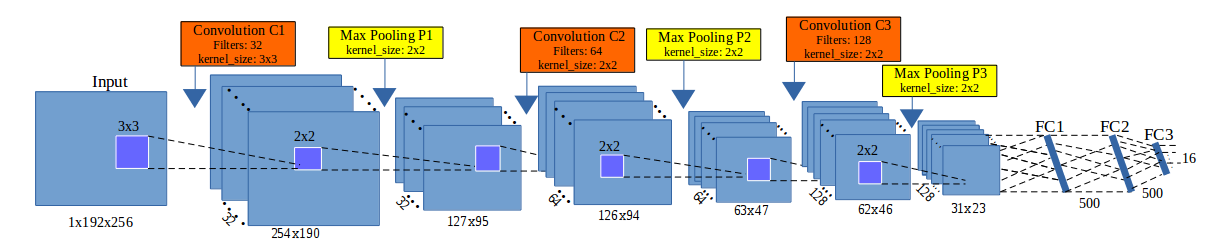
\includegraphics[scale=0.4]{images/net1}
	\caption{The architecture of the first model}
	\label{fignet1}
\end{figure}

The second architecture is modified from the first model. The layers are kept the same as the first one but the outputs of the first of two full-connected layers are changed from $500$ (in the first model) to $1000$ (Fig. \ref{}). Increasing the value at full-connected layers is hoping to obtain more features from convolutional layer and to prevent the over-fitting. 

\begin{figure}[h]
	\centering
	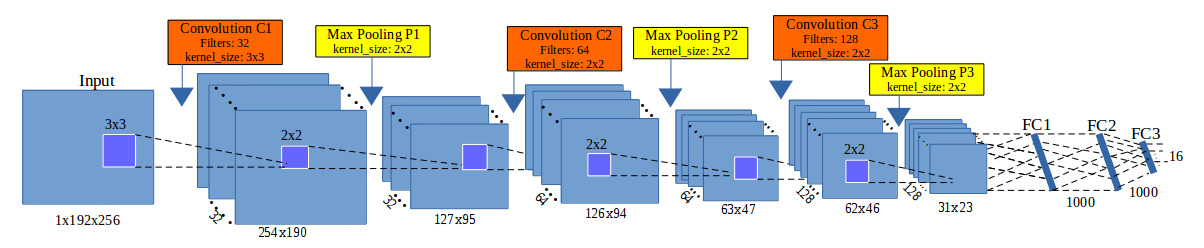
\includegraphics[scale=0.4]{images/net2}
	\caption{The architecture of the second model}
	\label{fignet2}
\end{figure}

To build the third architecture, we have used the definition of \textit{elementary block}. An {elementary block} is defined as a sequence of convolution ($C_{i}$), maximum pooling ($P_i$) and dropout ($D_i$) layers. This significantly reduces overfitting and gives major improvements over other regularization methods \cite{}. The idea of dropout is to include some variations between different runs. During training phase, dropout samples are done from an exponential number of different ``thinned” network. At test phase, it is easy to approximate the effect of averaging the prediction of all thinned networks by simply using a single unthinned network with smaller weights. So, we have modified the architecture by combining some \textit{elementary blocks}. Fig. \ref{fignet3} illustrates the layers in the third architecture. For our purpose, we have assembled \textbf{3 elementary blocks}. The parameters for each layer in each elementary block are as below, the list of values follows the order of elementary blocks ($i = [1..3]$):
\begin{itemize}
	\item CONV layers:
	\begin{itemize}
		\item Number of filters: $32, 64, $ and $128$
		\item Kernel filter sizes: $(3 \times 3), (2 \times 2), $ and $(2 \times 2)$
		\item Stride values: $1, 1, $ and $1$
		\item No padding is used for CONV layers 
	\end{itemize}
	\item POOL layers:
		\begin{itemize}
			\item Kernel filter sizes: $(2 \times 2), (2 \times 2), $ and $(2 \times 2)$
			\item Stride values: $2, 2, $ and $2$
			\item No padding is used for POOL layers
		\end{itemize}
	\item DROP layers:
		\begin{itemize}
			\item Probabilites: $0.1, 0.2, $ and $0.3$
		\end{itemize}
\end{itemize}

Three full-connected layers (FC) are kept the same as the second architecture: FC1 and FC2 have $1000$ outputs, the last full-connected layer (FC3) has $16$ outputs. As usual, a dropout layer is inserted between FC1 and FC2 with a probability equal to $0.5$.
\begin{figure}[h]
	\centering
	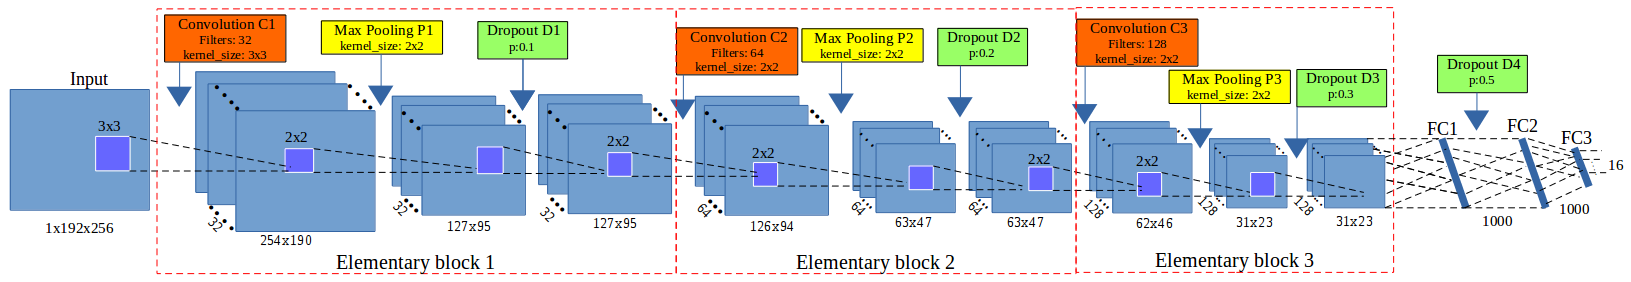
\includegraphics[scale=0.3]{images/arch_model}
	\caption{The architecture of the third model}
	\label{fignet3}
\end{figure}

The core of neural network is training over iteration. There are many ways to optimize the learning algorithm, but gradient descent \cite{} is currently a good choice to establish the way of optimizing the loss in neural network. The core idea is following the gradient until we statify with the results will remain the same. So, we have chosen gradient descent in the backward phase to update the values of learnable parameters and to increase the accuracy of the network. The networks are designed with a small sharing learning rate and a momentum. The learning rate is initialized at $0.03$ and stopped at $0.00001$, while the momentum is updated from $0.9$ to $0.9999$. Their values are updated over training time to fit with the number of epochs \footnote{An epoch is a single pass through the full training set}. The implementation of the architectures have been done on Lasagne framework \cite{} by Python. 

\section{Data augmentation}
A characteristic of machine learning and deep learning is using a volume dataset to train the model. Of course, in practice, we are not always have enough data for training. One way to solve this problem is to create the fake data from real data and to add it to the training set. Dataset augmentation has been a particularly effective technique for a specific problem. For example, in images classification problem, the operations like translating,  rotating or scaling the images have also effective. The fake images may be generated by translating (rotating or scaling) in each direction. Besides, injecting noise in the input can also see as a form of data augmentation.

Our dataset includes $293$ images of beetles (for each anatomical part). All the images are taken with the same camera in the same condition with a resolution of $3264 \times 2448$. Each image has a set of manual landmarks provided by biologists, i.e, each thorax has $8$ landmarks, each head has $10$ landmarks. Applying CNNs to train each part with a small number of images to reach good results is impossible. So, we need to augment the dataset before training the networks. Firstly, we have found that the original solution of the images $(3264 \times 2448)$ are heavy for the neural network. For performance considerations, in most of CNNs \cite{}, the size of the input is limited to $256 \times 256$ pixels, so we have decided to down-sampling the images to a new resolution $(256 \times 192)$ (to respect the ratio between $x$ and $y$). Of course, the coordinates of manual landmarks have been also scaled to fit with the new resolution of the images. In usual way, the transformations have been used to augment the dataset (i.e rotation, translation,\ldots) but the analysis of image by CNN is most often translation and rotation invariant. Therefore, two other procedures have been imaged to increase the number of images in the dataset $(256 \times 192)$.

The first procedure is to change the value of a color channel in the original image to generate a new image. According to that, a constant is added to one of the RGB channels each time it is used for training. Each constant is sampled in a uniform distribution $\in [1, N]$ to obtain a new value caped at $255$. For example, Fig. \ref{figaug1} shows an example when we added a constant $c = 10$ to each channel of an original image. Following this way, we can generate three version from an image.
\begin{figure}[h]
	\centering
	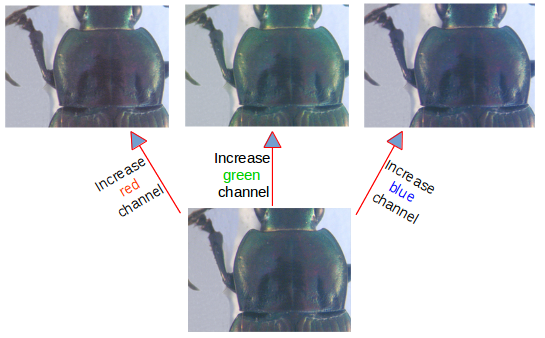
\includegraphics[scale=0.5]{images/inc_channels}
	\caption{A constant $c = 10$ has been added to each channel of an original image}
	\label{figaug1}
\end{figure}

In the second procedure, we have applied the opposite procedure to the first one. Instead of adding the value, we separate the channels of RGN into three gray-scale images as the network works on single channel images. At the end of the processes, we are able generate six versions from an original image. In total, we have $293 \times 7 = 2051$ images for each anatomical part of beetle (an original image and six generated images). However, we have not used all images for training and validation. So, we have chosen $260$ original images and their generations ($1820$ images) of each dataset for training and validation processes, the remaining images ($33$ original images) are used for test process.

\begin{figure}[h]
	\centering
	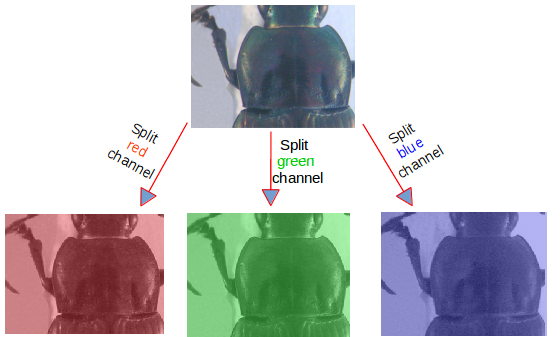
\includegraphics[scale=0.5]{images/sp_channels}
	\caption{Three channels (red, green, blue) are separated from original image}
	\label{figaug2}
\end{figure}

In practical, to obtain a fast convergence during the computing, it is useful to normalize the brightness of the images to $[0,1]$ instead of $[0, 255]$ and the coordinates of the landmarks have been also normalized. 
\section{Experiments and results}
Before widely applying to all anatomical parts, we have firstly tried with thorax part to evaluate the performance. The networks have been trained in $5, 000$ epochs on Ubuntu machine by using NVIDIA TITAN X cards. The set of images that used for training and validation are merged together. 

During the training, the images are chosen randomly from the dataset with a ratio of $60\%$ for training and $40\%$ for validation. The training step takes into account a pair of information (\textit{images, manual landmarks coordinates})  as training data. In the context of deep learning, landmark prediction can be seen as a regression problem. So, we have used Root Mean Square Error (RMSE) to compute the loss of implemented architectures.

At the test phase, images without landmarks are given to the trained network to produce output coordinates of the predicted landmarks. The results then evaluated by comparing with the manual landmarks coordinates provided by biologists which have been seen as ground truth. Fig. \ref{figloss1} shows the training errors and the validation errors during traning phase of the first architecture. The blue curve presents the RMSE errors of training process, the green curve presents the validation errors. Clearly, over-fitting has appeared in the first model. The training losses are able to decrease but the validation losses are stable. In the second model (section \ref{}), we have modified the parameters of full-connected layers to prevent the over-fitting but it seems that this solution is still not suitable. The over-fitting is also appeared as the first model.

\begin{figure}[h]
	\centering
	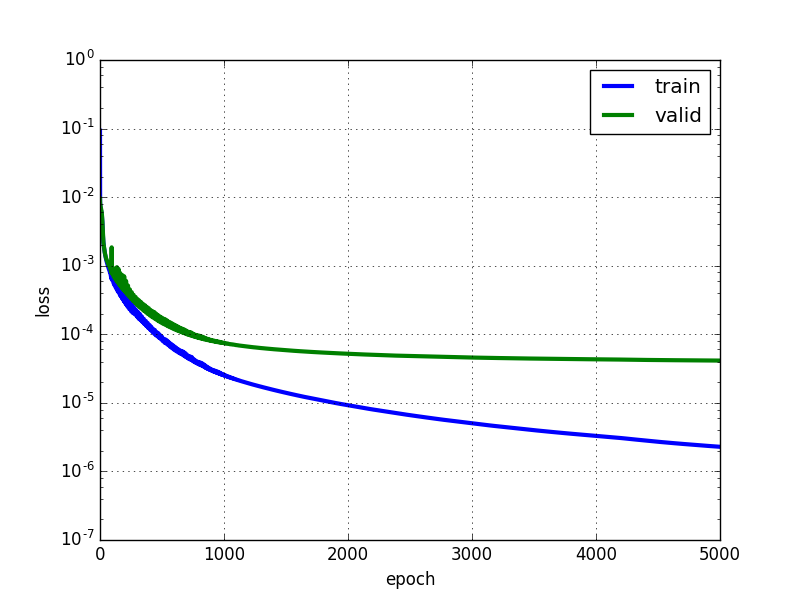
\includegraphics[scale=0.6]{images/cnnmodel3_5000_pronotum_v13_without_dropout_normalized_data_loss}
	\caption{The training and validation losses of the first model}
	\label{figloss1}
\end{figure}

Then, we have continued to train the third model on the same dataset of thorax images. Fig. \ref{figloss2} illustrates the losses during the training of the third model. Like the previous figure (Fig. \ref{figloss1}), the blue line is training losses, the green line is validation losses. In the opposite with two previous models, the losses are different (far) from the beginning but after several epochs, the values become more proximate and the over-fitting problem has been solved. This proves that adding dropout layers to build the elementary blocks have been effects to prevent over-fitting and contributory improve the accuracy of the model. \textit{So, we have decided to keep the architecture of the third model for our landmarking problem.}

\begin{figure}[h]
	\centering
	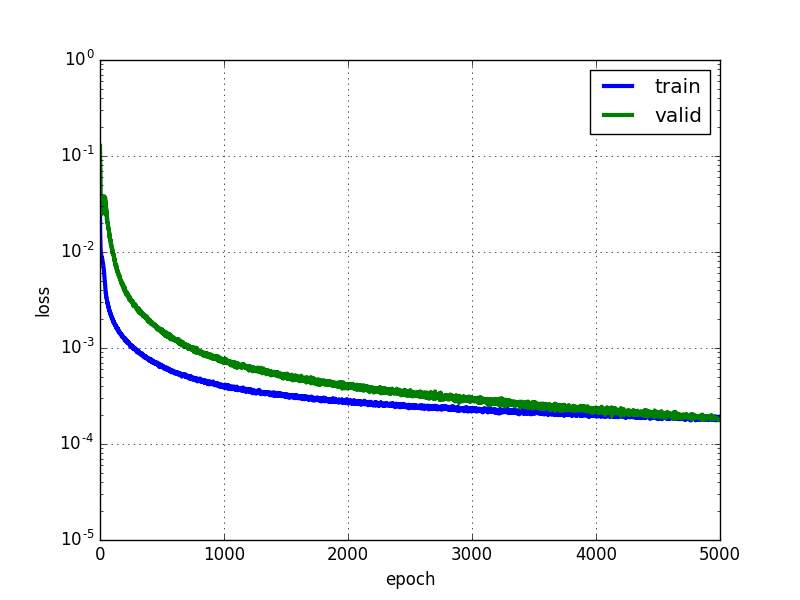
\includegraphics[scale=0.6]{images/loss_v16}
	\caption{The training and validation losses of the third model}
	\label{figloss2}
\end{figure}

In order to have the predicted landmarks for all thorax images (instead of only $33$ images), we have applied \textit{cross-validation} to choose the test images, called \textit{round}. For each time, we have chosen a different fold of $33$ images as testing images, the remaining images are used as training and validation images ($293/33 \approx 9$ rounds). Following that, the network will be trained with many different datasets, then the trained model will be used to predicted the lanmarks on the images in the corresponding test set. Table. \ref{tbltrainingloss} resumes the losses of $9$ rounds when we trained the third model on thorax images.

\begin{table}[h!]
	\centering
	\begin{tabular}{l l l}
	Round & Training loss & Validation loss \\ \hline
	1 & 0.00018 & 0.00019  \\ \hline
	2 & 0.00019 & 0.00021 \\ \hline
	3 & 0.00019 & 0.00026 \\ \hline
	4 & 0.00021 & 0.00029 \\ \hline
	5 & 0.00021 & 0.00029 \\ \hline
	6 & 0.00019 & 0.00018 \\ \hline
	7 & 0.00018 & 0.00018 \\ \hline
	8 & 0.00018 & 0.00021 \\ \hline
	9 & 0.00020 & 0.00027 \\ \hline
	\end{tabular}
	\caption{\small{The losses during training the third model on thorax images}}
	\label{tbltrainingloss}
\end{table}

To evaluate the coordinates of predicted landmarks, the correlation metrics have been computed the correlation between the manual landmarks and their corresponding predicted one. Table. \ref{tblcorrelation} shows the correlation scores of $3$ metrics (using \textit{scikit-learn} \cite{}), i.e, coefficient of determination ($r^2$), explained variance (EV), and Pearson correlation. All of three metrics have the same possibility. The best score is $1.0$ if the correlation data is good, lower values are worse. It means that our predicted coordinates are very close with the ground truth. However, the measure is not enough good to provide a useful result to biologists. Moreover standing on the side of image processing, we are looking forward to  seeing the predicted coordinates than the statistical results.

\begin{table}[htbp]
	\centering
	\begin{tabular}{|c|p{2cm}|p{2cm}|p{2cm}|}
		Metric & $\mathbf{r^{2}}$ & \textbf{EV} & \textbf{Pearson} \\ \hline
		Score & $\textbf{0.9952}$ & $\textbf{0.9951}$ & $\textbf{0.9974}$ 
	\end{tabular}
	\caption{Correlation scores between manual landmarks and predicted landmarks}
	\label{tblcorrelation}
\end{table}

The main goal of computing is to predict the coordinates of landmarks, so the distances (in pixels) between the coordinates of manual landmarks and corresponding predicted landmarks have been taken into account on all images. Then, the average of distances are computed by landmarks. Table. \ref{} shows the average distances by landmarks on all images of thorax dataset. With images of resolution $256 \times 192$, we can
consider that an error of $1\%$ corresponds to $2$ pixels that could
be an acceptable error. Unhappily, our results exhibit average
distance of $4$ pixels in the best case, landmark $1$ and more than
$5$ pixels, landmark $6$. Other error distances are more than $2\%$
pixels.

\begin{table}[htbp]
	\centering
	\begin{tabular}{|c|c|}
		\hline
		\textbf{Landmark} & \textbf{Distance} (in pixels) \\ \hline
		1 & 4.002  \\ \hline
		2 & 4.4831 \\ \hline
		3 & 4.2959 \\ \hline
		4 & 4.3865 \\ \hline
		5 & 4.2925 \\ \hline
		6 & 5.3631 \\ \hline
		7 & 4.636 \\ \hline
		8 & 4.9363 \\ \hline
	\end{tabular}
	\caption{The average distances on all images per landmark.}
\end{table}

Fig. \ref{figchartlm1} shows the distribution of the distances on the first landmark of all images. The accuracy based on the distance in each image can be
separated into three spaces: the images have the distance less
than average value ($4$ pixels): $56.66\%$; the images have the
distance from average value to $10$ pixels (average distance plus
standard deviation): $40.27\%$; and the images have the distance
greater than $10$ pixels: $3.07\%$.

\begin{figure}[htbp]
	\centerline{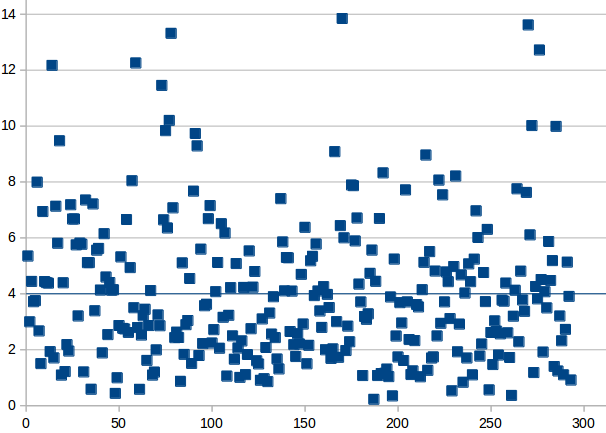
\includegraphics[scale=0.5]{images/statistic_pronotum_from_scratch_lm1}}
	\caption{The distribution of the distances on the first landmark. The blue line is the average value of all distances.}
	\label{figchartlm1}
\end{figure}

To illustrate this purpose, Fig. \ref{figrsexample} shows the predicted landmarks on two test images. One can note that even some predicted landmarks (Fig. \ref{figsub1}) are closed to the manual ones, in some case (Fig. \ref{figsub2}) the predicted ones are far from the expect results. The next step has been dedicated to the improvement of these results.

\begin{figure}[htbp]
    \centering
    \subfloat[Image with well-predicted landmarks]{\label{figsub1}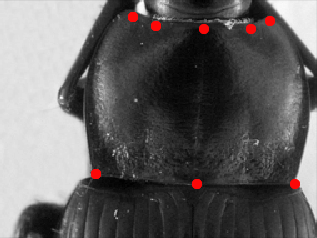
\includegraphics[width=0.45\textwidth]{images/fn_accuracy}}~~
\subfloat[Image with inaccuracy landmarks]{\label{figsub2}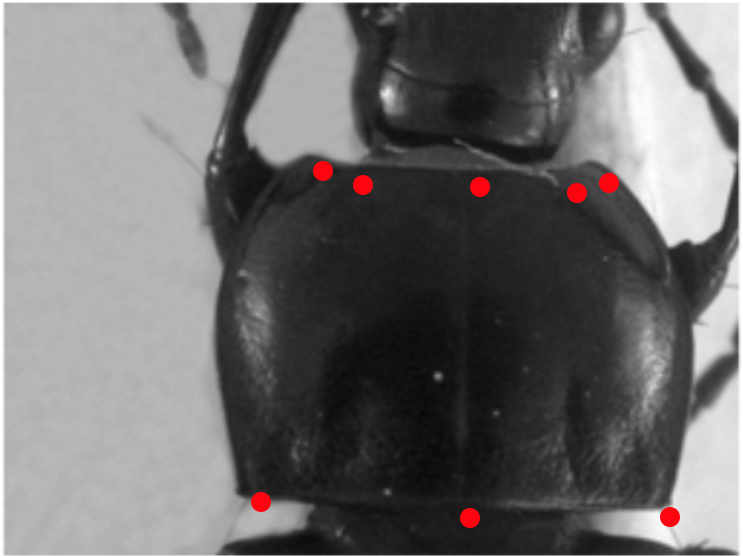
\includegraphics[width=0.45\textwidth]{images/plandmark2}}\\    
    \caption{The predicted landmarks, in red,  on the images in test set.}
    \label{figrsexample}
\end{figure}

\textbf{How about the results on head and elytra parts???????}
\section{Conclusion}


\iffalse

\section{Model 1: Facial point detection by CNN}
Yi Sun et al\cite{sun2013deep} focused on five facial keypoints: \textit{left eye center}(LE), \textit{right eye center}(RE), \textit{nose tip}(N), \textit{left mouth corner}(LM) and \textit{right mouth corner}(RM) (called landmarks). A model with 3-levels of networks are proposed to study from high-level to low-level of the landmarks.
\subsection{Data}
The dataset with 13466 face images includes 5590 images from LFW \cite{huang2007labeled} and remaining images are downloaded from the web. The dataset is randomly divided into the training set with 10000 images and validation set with 33466 images. Each face is labeled with five landmarks and the bounding box is created around the face.
\subsection{Architecture}
The proposed architecture includes 3-levels of CNN: three networks at the first level, and ten networks for each remaining level(Fig.\ref{3levels}). The networks at level 1 is designed to detect multiple landmarks while two last levels are designed for working on each landmark.
\begin{figure}[h]
	\centering
	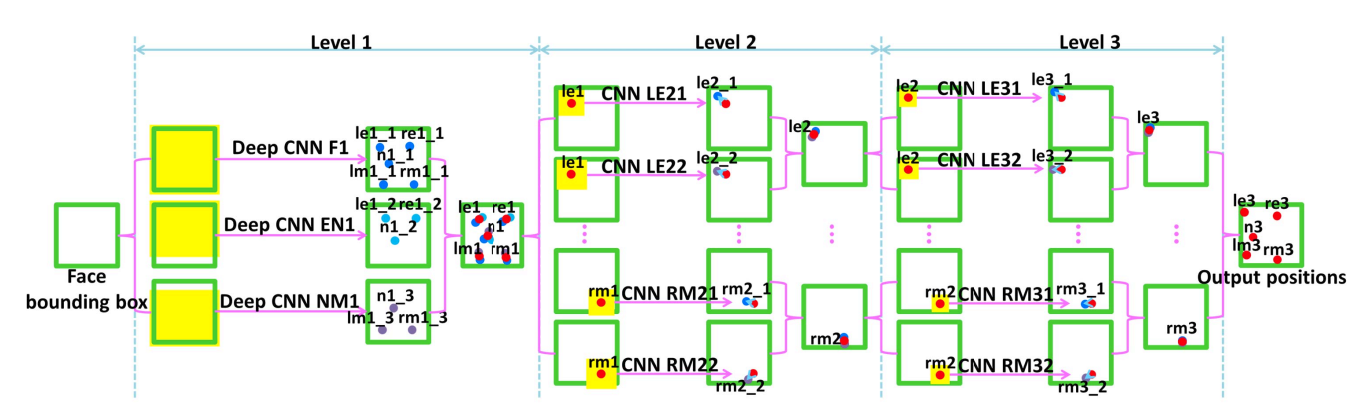
\includegraphics[scale=0.35]{images/3levels}
	\caption{The 3-levels proposed architecture}
	\label{3levels}
\end{figure}

At the first level, three CNNs are employed to study the location of the facial points: F1, EN1, NM1 whose input regions cover the whole face. F1 is studied all the position of five landmarks; EN1 is worked on the eyes and nose while NM1 worked on nose and the mouth corners. Each network predicts the landmarks corresponding with the region that it covers. At the end of level 1, the coordinate of each landmark is averaged of coordinates that predicted from three networks. Fig.\ref{1Fconv} illustrates the deep structure of the networks at level 1, which contains four convolutional layers followed by max pooling and two dense layers. F1, EN1, and NM1 take the same structure but with different size of the input and different output at full-connected layers to suitable with the number of predicted landmarks.
\begin{figure}[h]
	\centering
	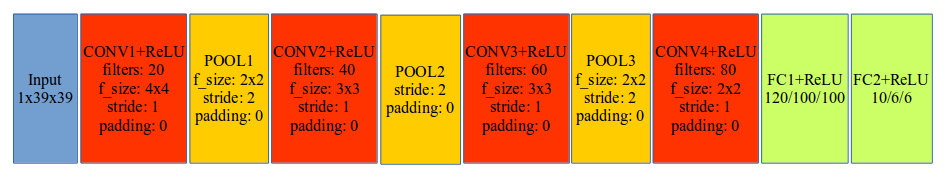
\includegraphics[scale=0.5]{images/cnn_level1}
	\caption{The structure of the networks in level 1}
	\label{1Fconv}
\end{figure}

The networks at the second and third levels take local patches centered at the predicted position of previous levels as input. Besides, they allowed to make small changes to previous prediction. The size of patches are also reduced along with the cascade model. For each position, two networks are used to predict the new positions. The last predicted position is average of the new positions. Fig.\ref{2lvconv} illustrates the architecture of the networks in level 2 and level 3. Basically, the networks in last two levels are similar, the only difference is the way to choose the patch around the landmark. A padding is added to the coordinates of the landmark to make the change of the patches i.e $0.16, 0.18$ in level 2 and $0.11, 0.12$ in level 3. Then, the patch is resized to the size of $15 \times 15$ before giving the networks.
\begin{figure}[h]
	\centering
	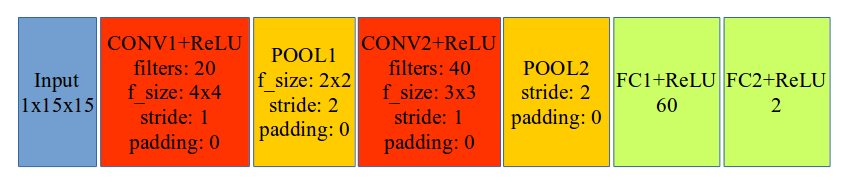
\includegraphics[scale=0.5]{images/cnn_level2}
	\caption{The structure of the networks in level 2, level 3}
	\label{2lvconv}
\end{figure}

 With 3-levels model, the purpose of the networks at the first level are estimated the landmark positions with large errors; the networks at last two levels are designed to achieve high accuracy.
\subsection{Experiments}
\subsubsection{Training}
At the first level, $F1$ takes the whole face as input (size of $39 \times 39$ of the network and outputs the position of all the five points. $EN1$ takes the top and middle part of face as input (size of $31 \times 39$) and outputs the positions of two eye centers and nose tip. $NM1$ takes the bottom and middle part of the face to predict the positions of nose tip and two corners of mouth.

All the networks at level 2 and level 3 take a small squares ($15 \times 15$)centered at the predicted position by the previous level as the input and output the incremental prediction. The last predicted positions at each level are average of corresponding positions from all the networks in each level. 

During training, the size of the patches is decreased for each level. The learnable parameters include weight w, the gain g and the bias b which are initialized by small random number and learned by stochastic gradient descent.

The detection error on each facial point is measured by Eq.\ref{eq1}. If the error is greater than $5\%$, it is considered as failure.
\begin{equation}
	err = \sqrt{(x-x')^2 + (y-y')^2}/l
	\label{eq1}
\end{equation}
Where:
\begin{itemize}
	\item l is the width of the bounding box around the face.
	\item $(x,y)$ is ground truth facial point
	\item $(x',y')$ is predicted position
\end{itemize}
\subsubsection{Testing}
The model is tested with a dataset of 2557 face images. The image with the bounding box of the face is used as the input of the model. At the end, the predicted position is estimated from the model. By using the way in Eq.(\ref{eq1}) to evaluate the model, the error statistic on each level is obtained (Figs. \ref{rslevel1}, \ref{rslevel2}, \ref{rslevel3}).
%\begin{table}[h!]
%	\centering
%	\begin{tabular}{c}
%	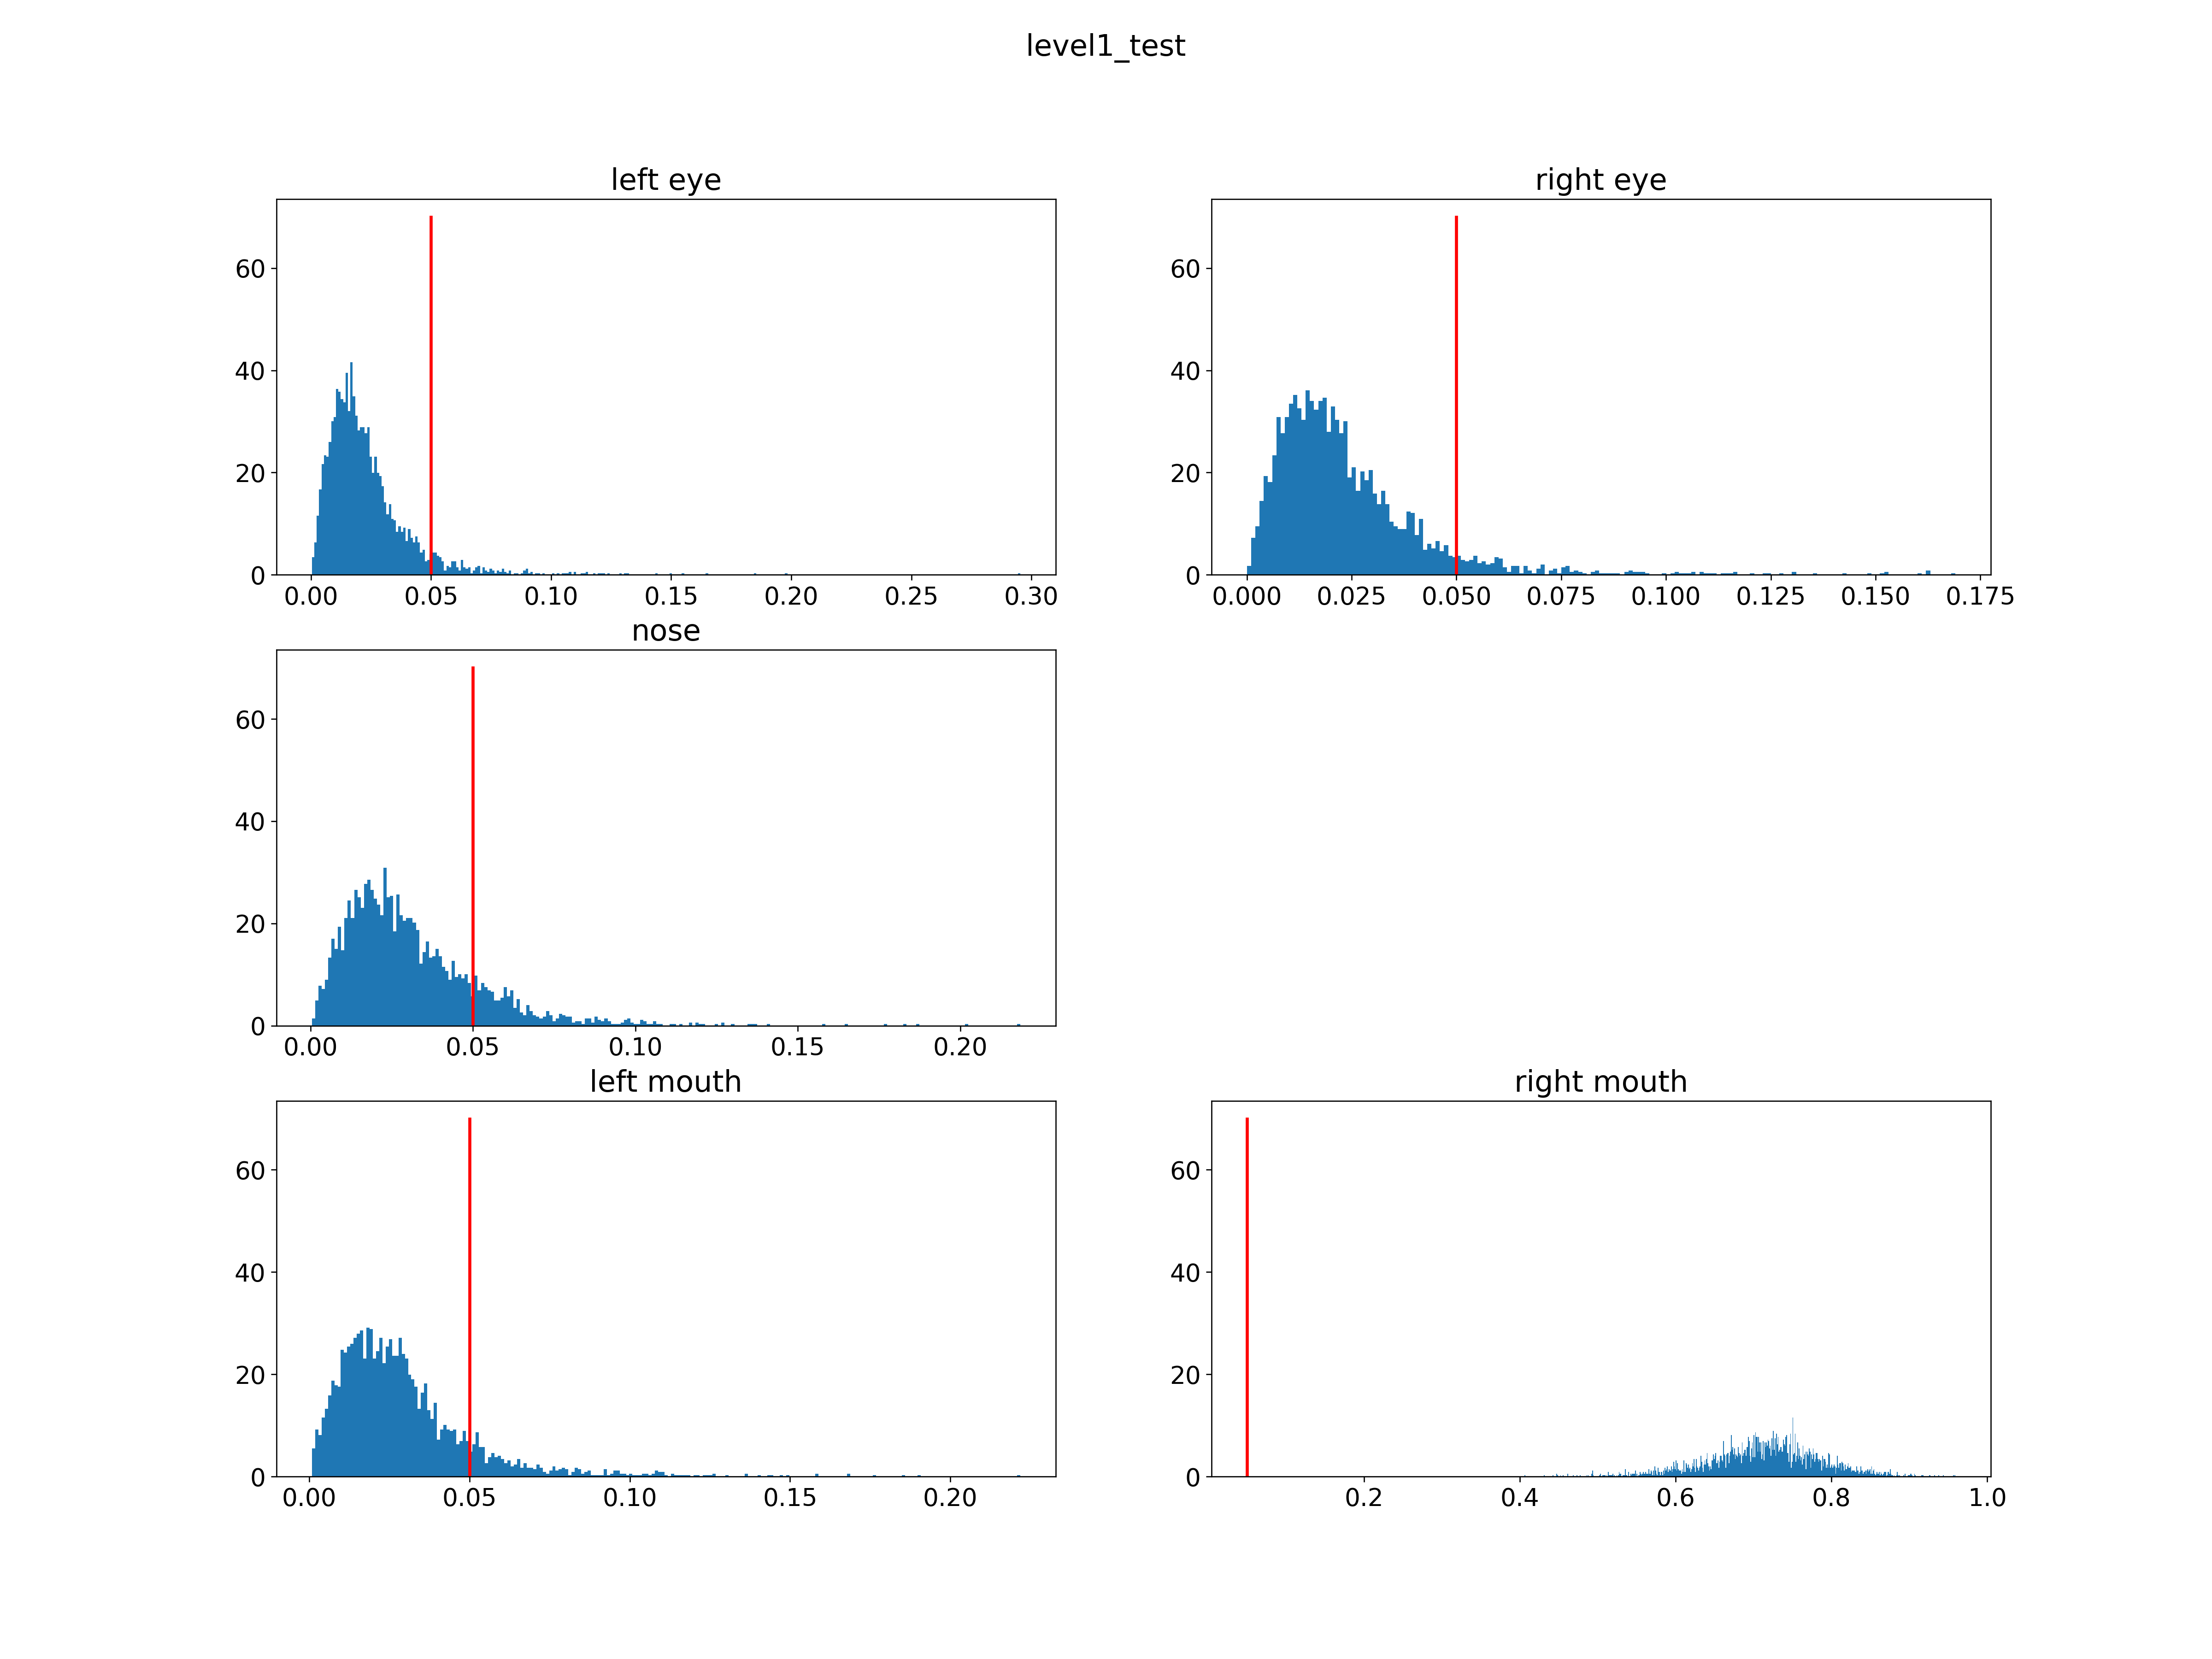
\includegraphics[scale=0.3]{images/level1_test}~\\
%	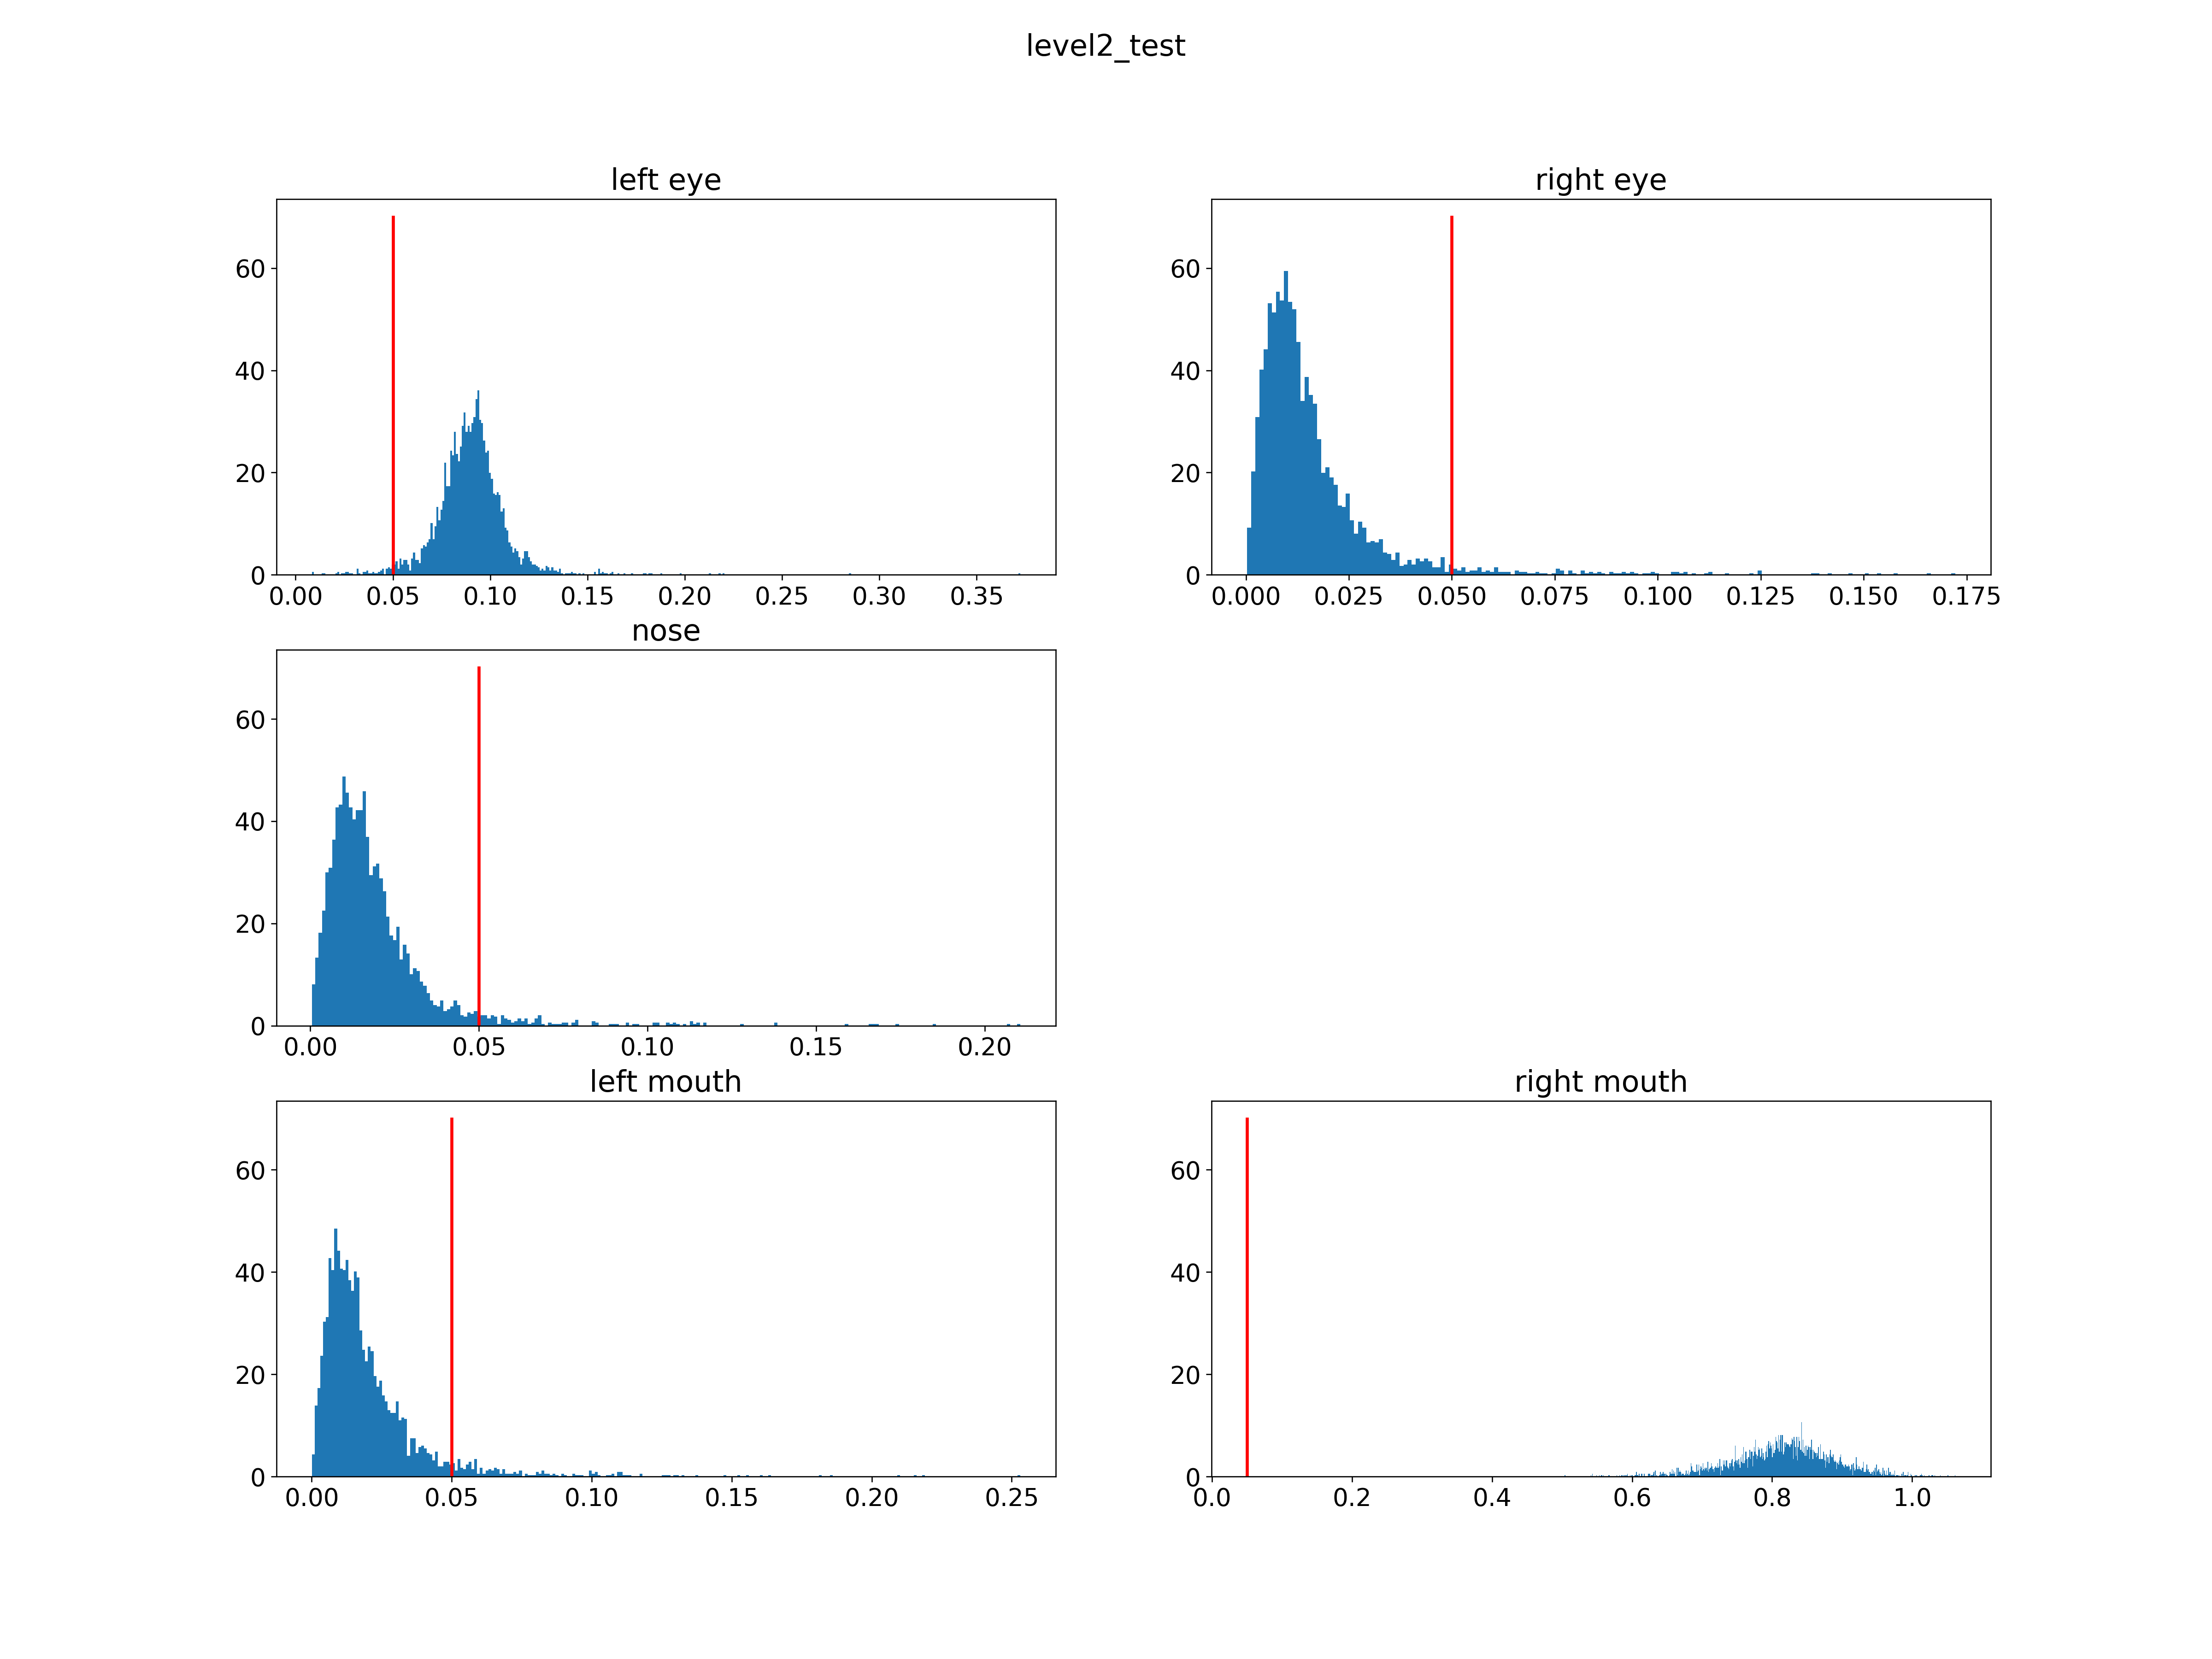
\includegraphics[scale=0.3]{images/level2_test}~\\
%	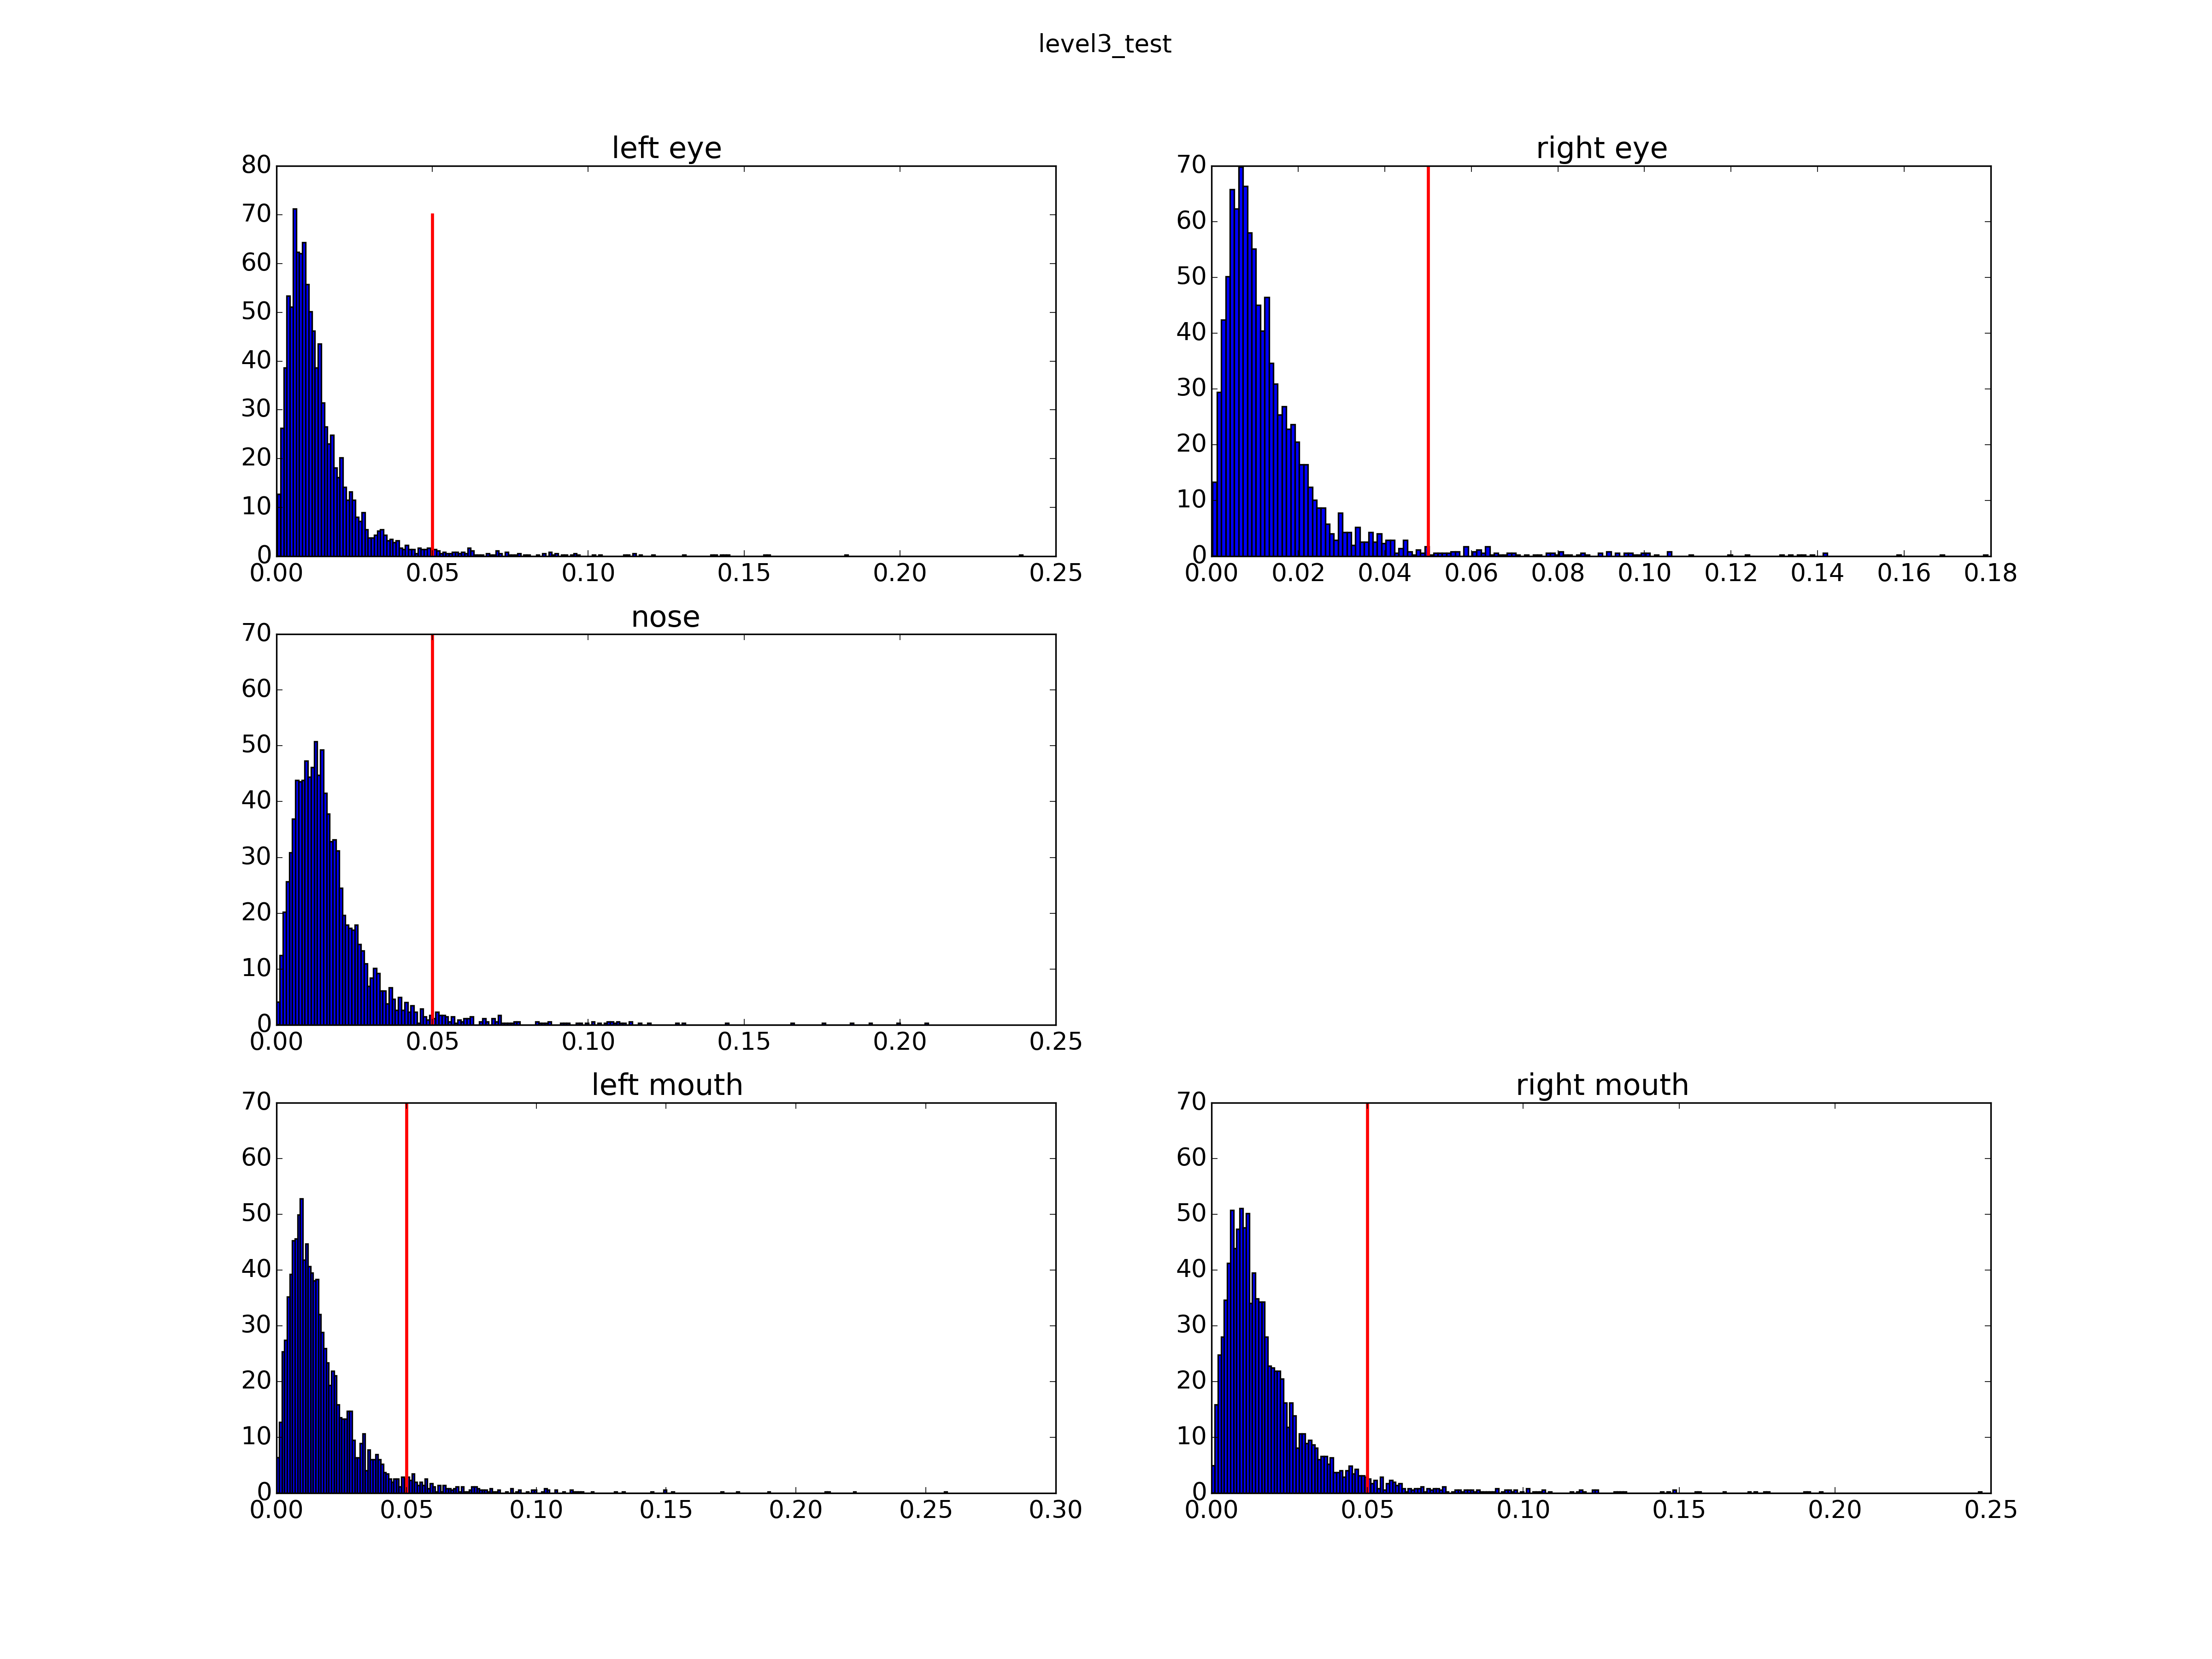
\includegraphics[scale=0.3]{images/level3_test}
%	\end{tabular}	
%\end{table}
\begin{figure}[h!]
	\centering
	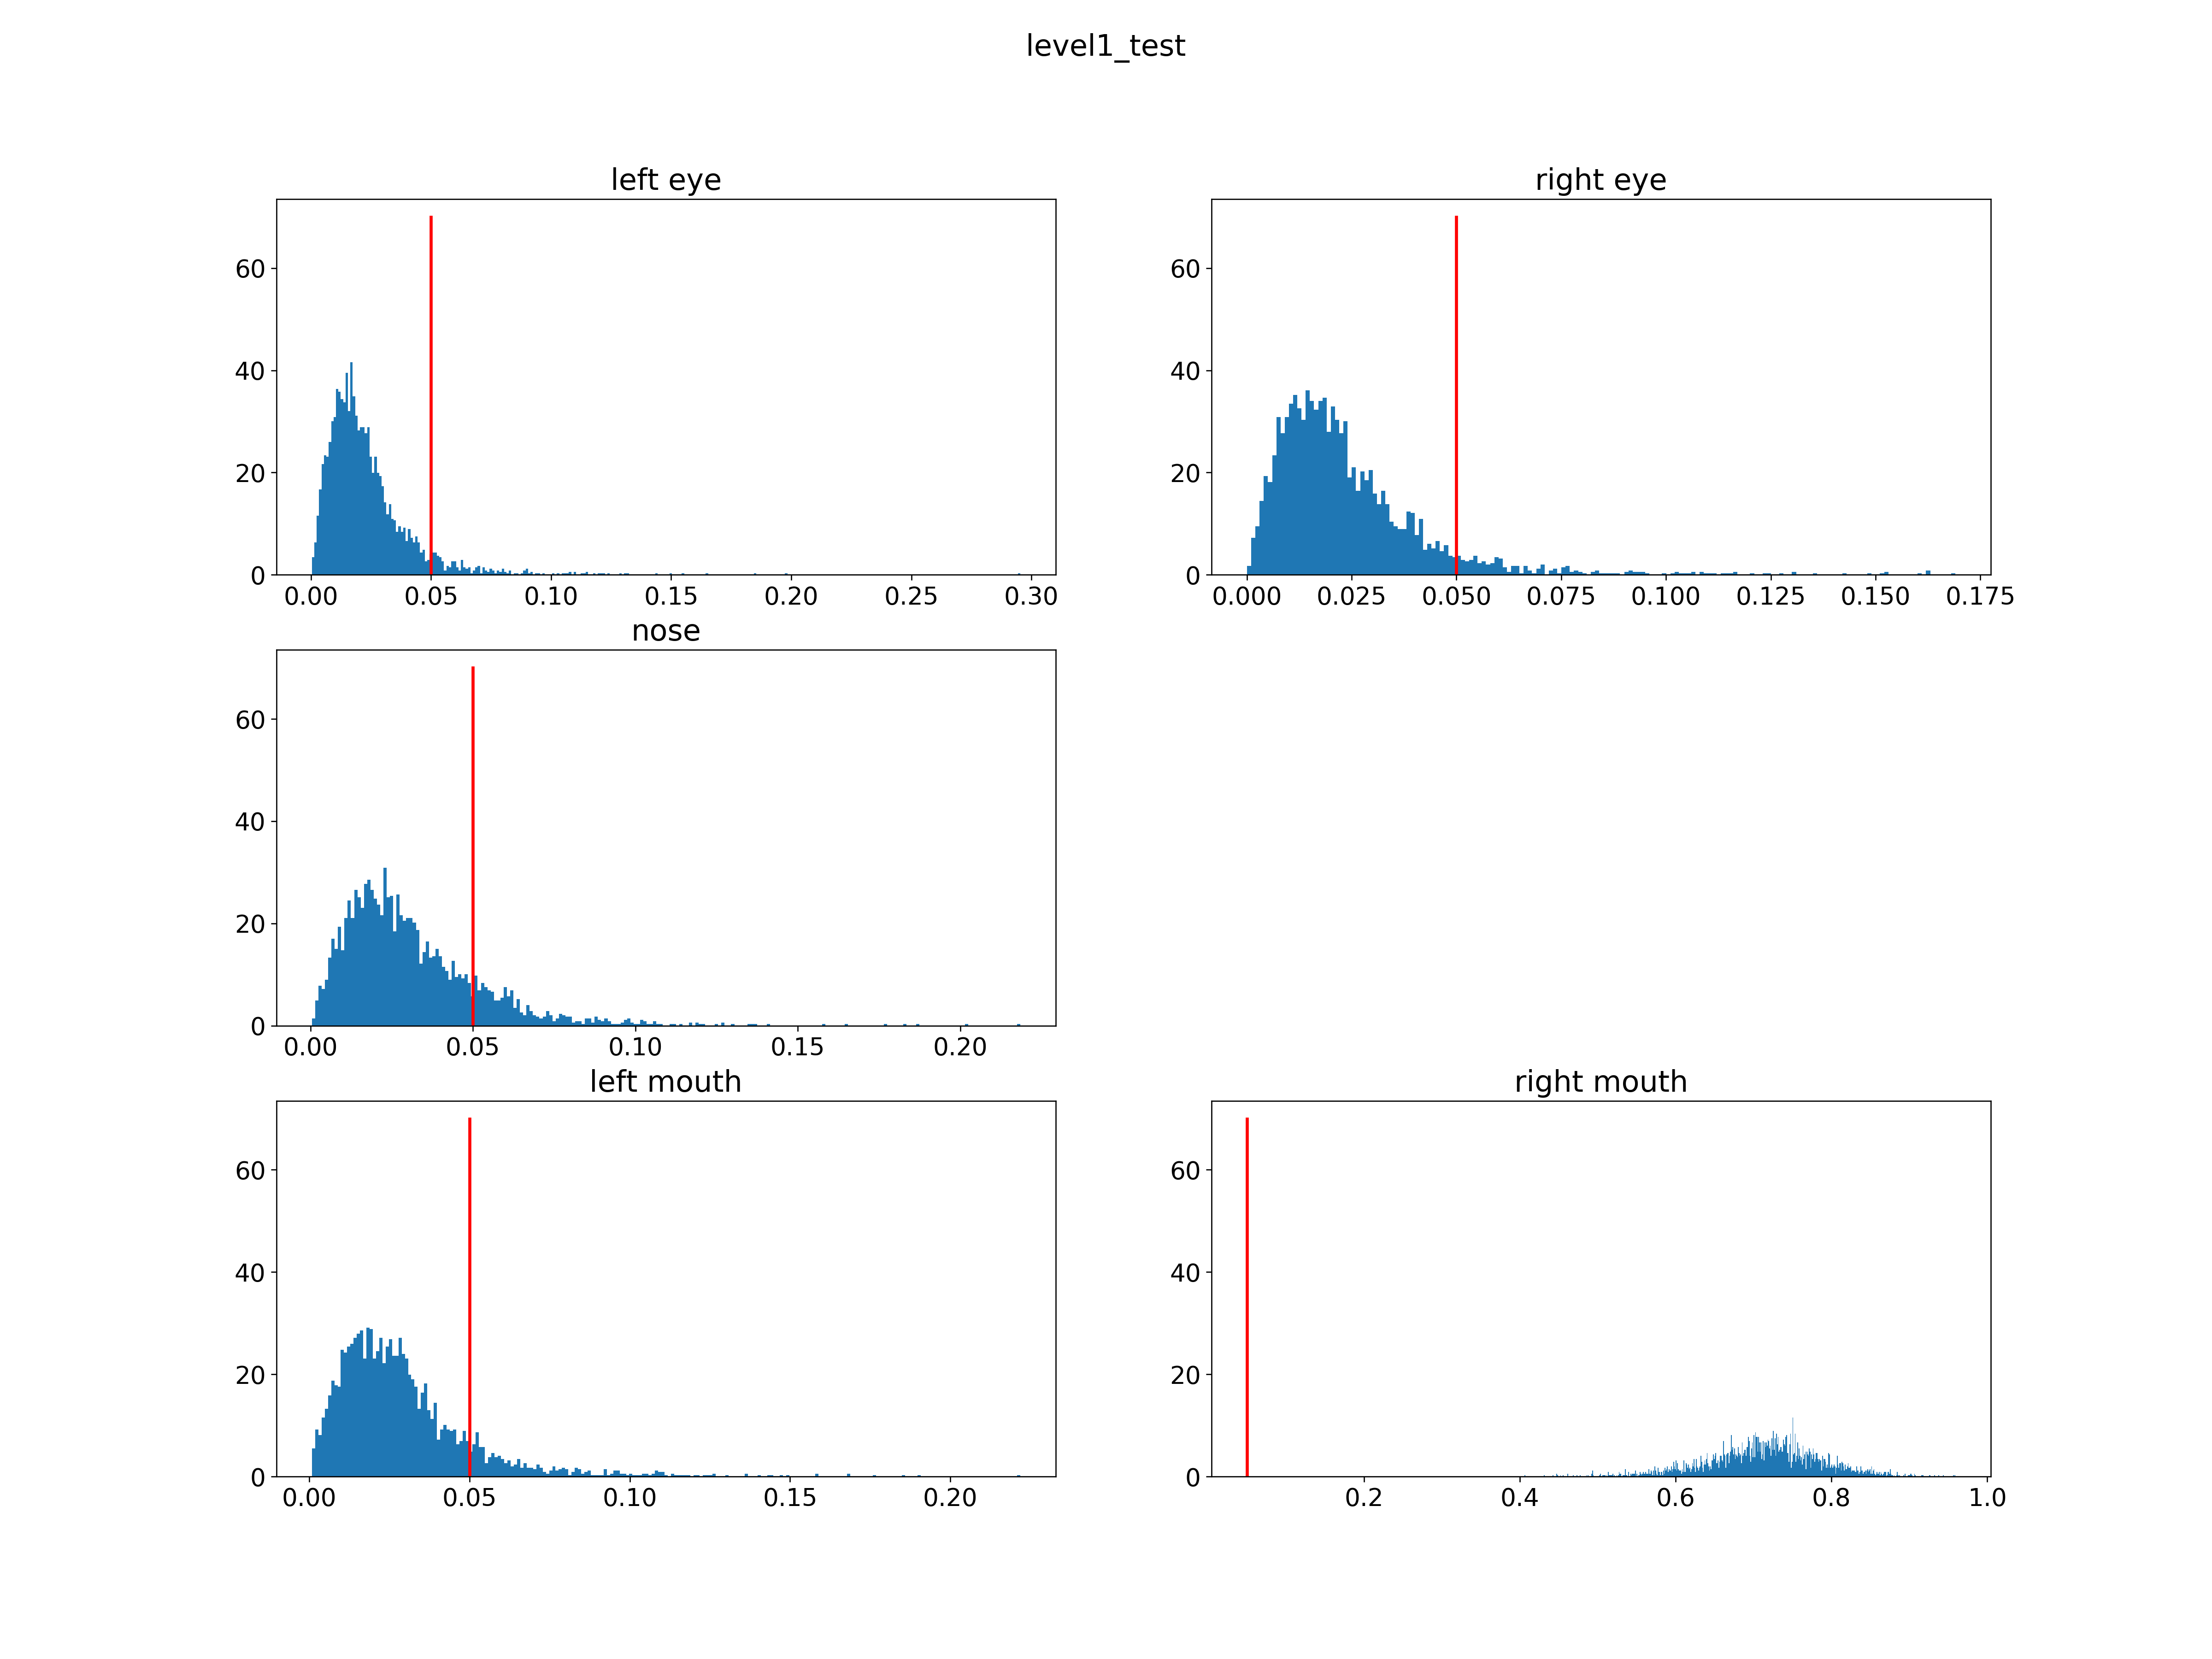
\includegraphics[scale=0.25]{images/level1_test}
	\caption{The error on each landmark in level 1}
	\label{rslevel1}
\end{figure}
\begin{figure}[h!]
	\centering
	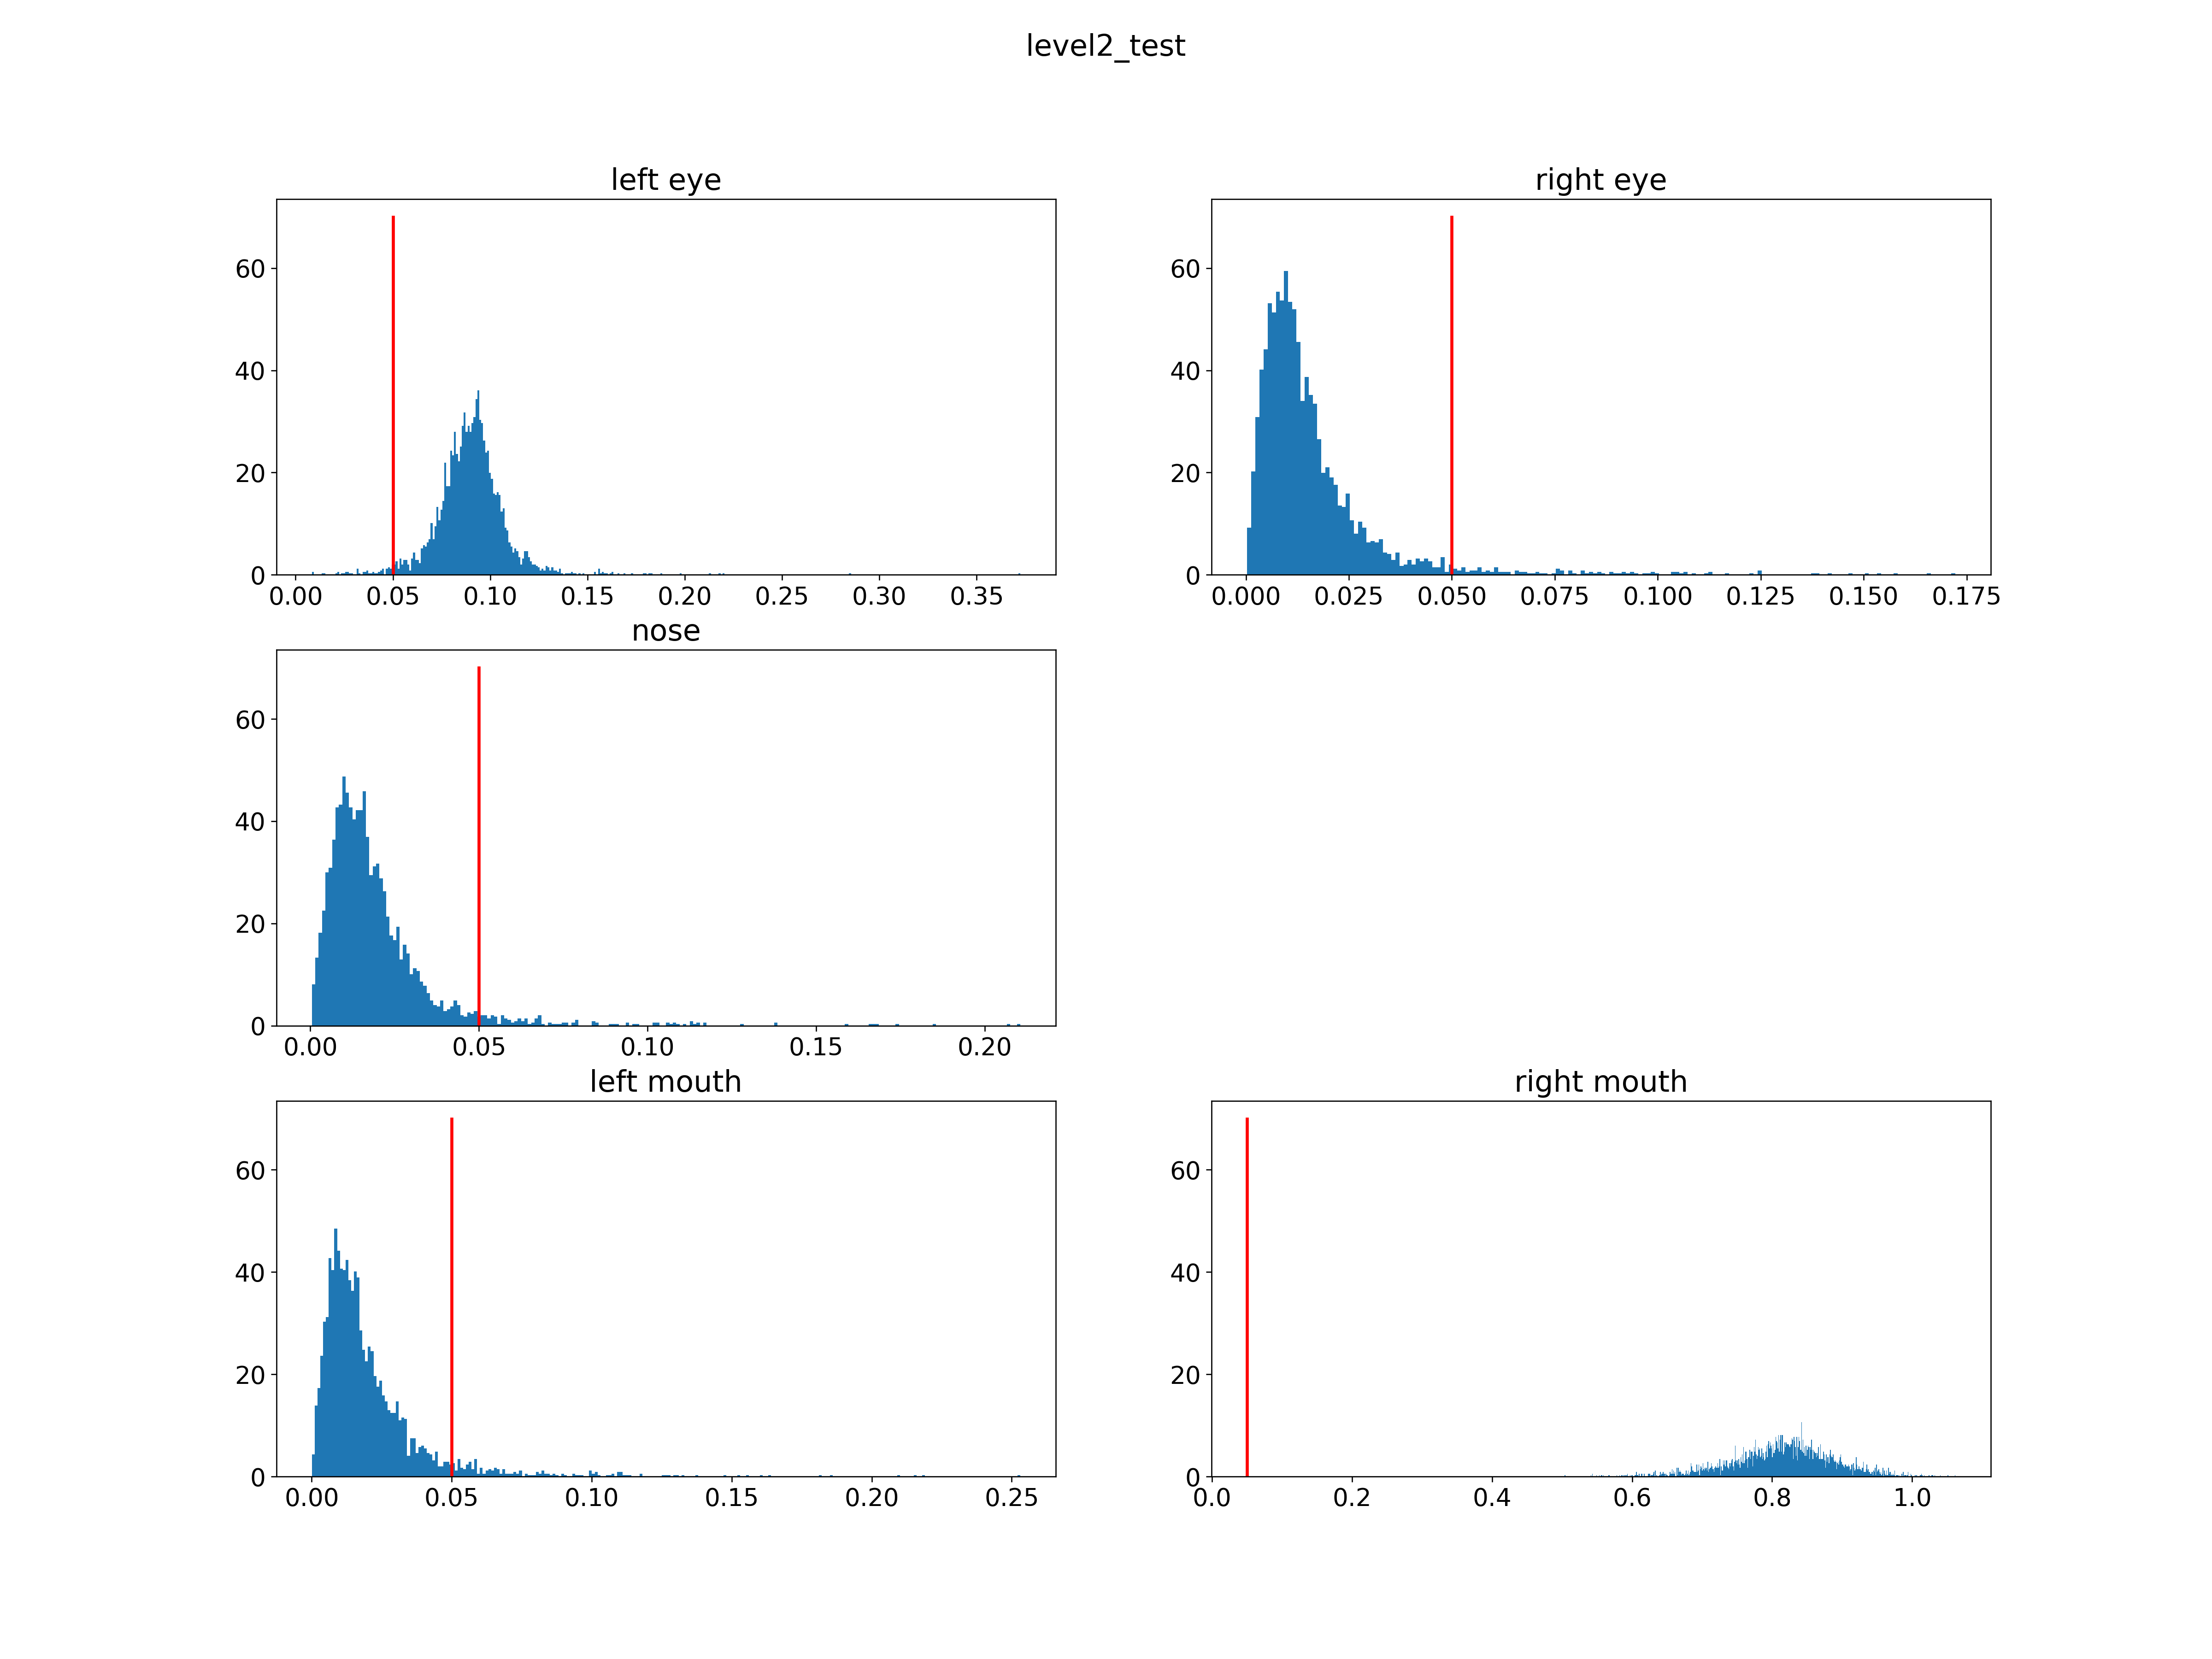
\includegraphics[scale=0.25]{images/level2_test}
	\caption{The error on each landmark in level 2}
	\label{rslevel2}
\end{figure}
	\begin{figure}[h!]
	\centering
	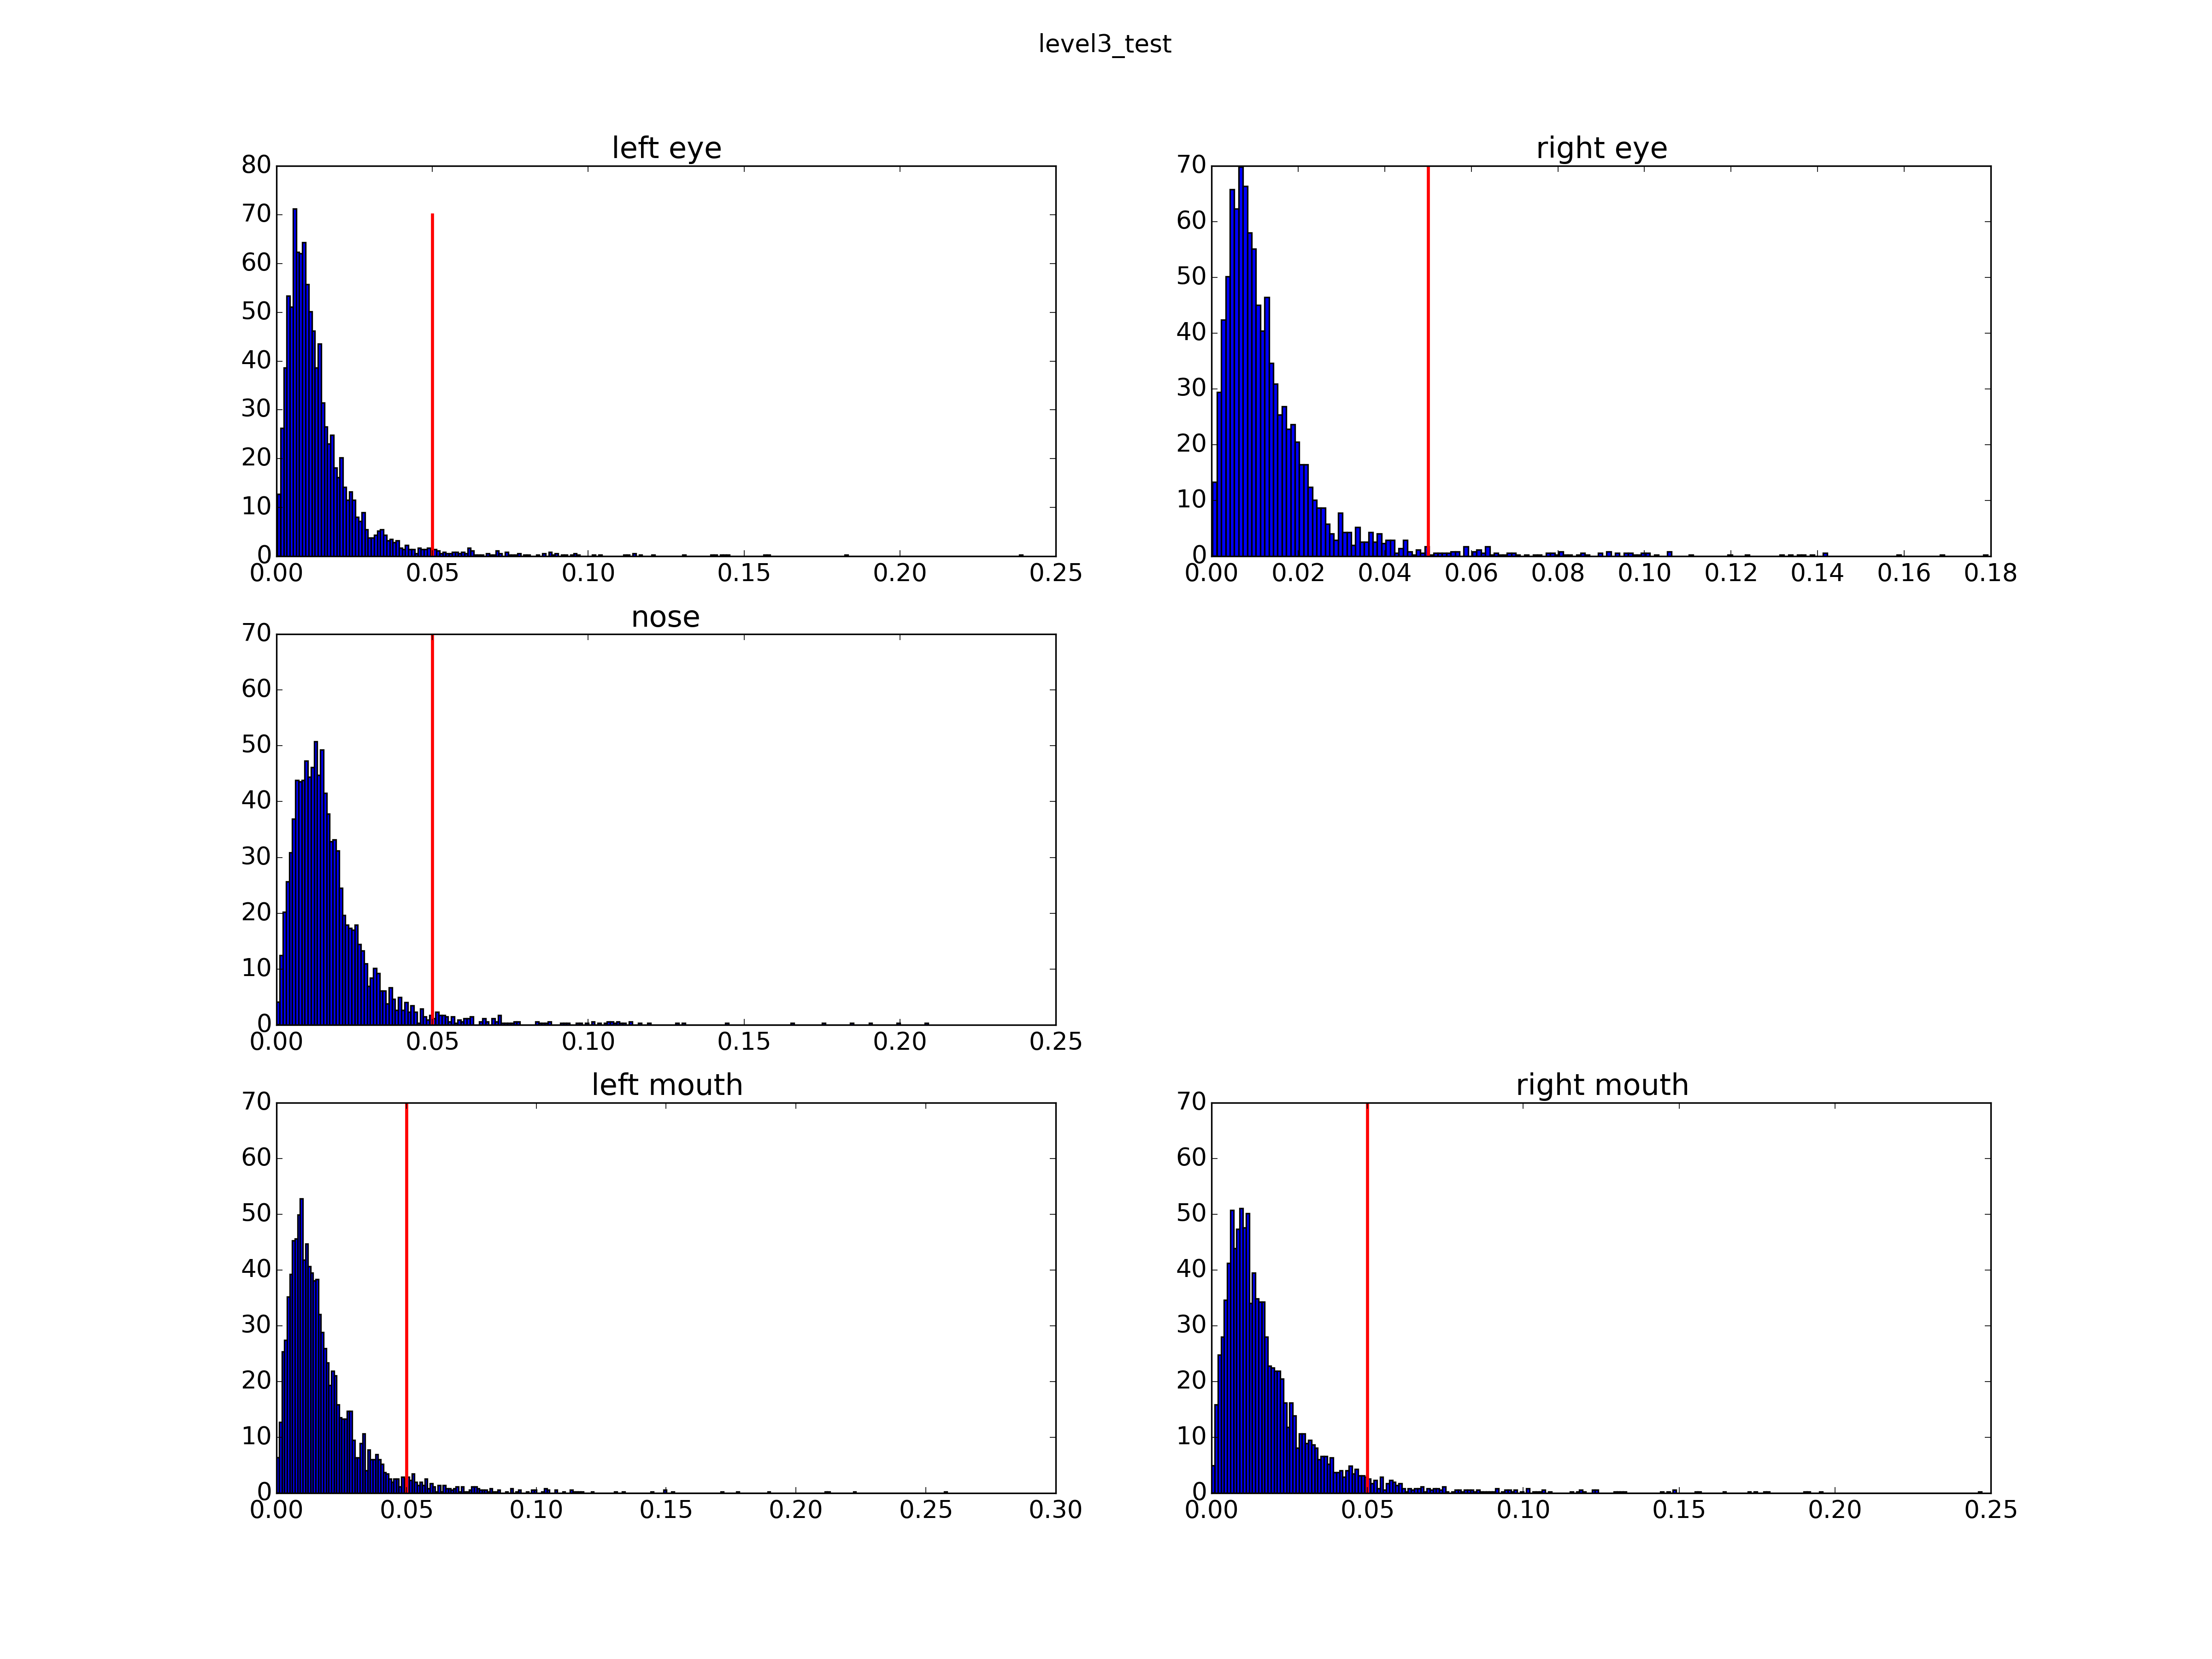
\includegraphics[scale=0.25]{images/level3_test}
	\caption{The error on each landmark in level 3}
	\label{rslevel3}
\end{figure}
\pagebreak
\section{Model 2: Automatic ear landmarks detection by CNN}
Celia Cintas et al\cite{cintas2016automatic} proposed a method based on geometric morphometric and deep learning for automatic ear detection and feature extraction in the form of landmarks. The convolutional neural network was trained with a set of manually landmarks examples. The network is able to provide the morphometric landmarks on ear image automatically.
\subsection{Dataset}
The image and manual landmarks belong to the CANDELA initiative \footnote{https://www.ucl.ac.uk/candela}, a project includes geneticists, bioinformatics and social-anthropologists interested on Latin American. CANDELA contains 7500 images with the size of $2136 \times 3216$. The provided dataset contains 2753 images which extracted from the CANDELA dataset. For each image, a set of 45 landmarks and semi-landmarks provided by human operators. The dataset was split into a training set with 2051 images (75\%) and a validation set of 684 images (25\%).
\subsection{Network}
Three models were designed and trained for performing the automatic landmarks task. These architectures are different in the number of convolution layers, the filter sizes, and the learning rate. An image with a single channel of the size  $96 \times 96$ with brightness scaled to $[0,1]$, is taken as the input of the network. The target (landmarks coordinates) is scaled to $[-1,1]$. \textbf{Fig.\ref{1Econv}} shows the best architecture. In this architecture, a structure of two convolutional layers with the filters, followed by maximum pooling and dropout layer. This structure is repeated three times to obtain features at different levels with different size of filters(i.e $4 \times 4$ and $3 \times 3$). After extraction the features, two fully connected linear layers with 1500 units each and a dropout layer is hired. The output layer contains 90 output units corresponding with 45 landmarks for the predicted position of the landmarks. The implementation used Python and the Lasagne library\cite{lasagne}.
\begin{figure}[h!]
	\centering
	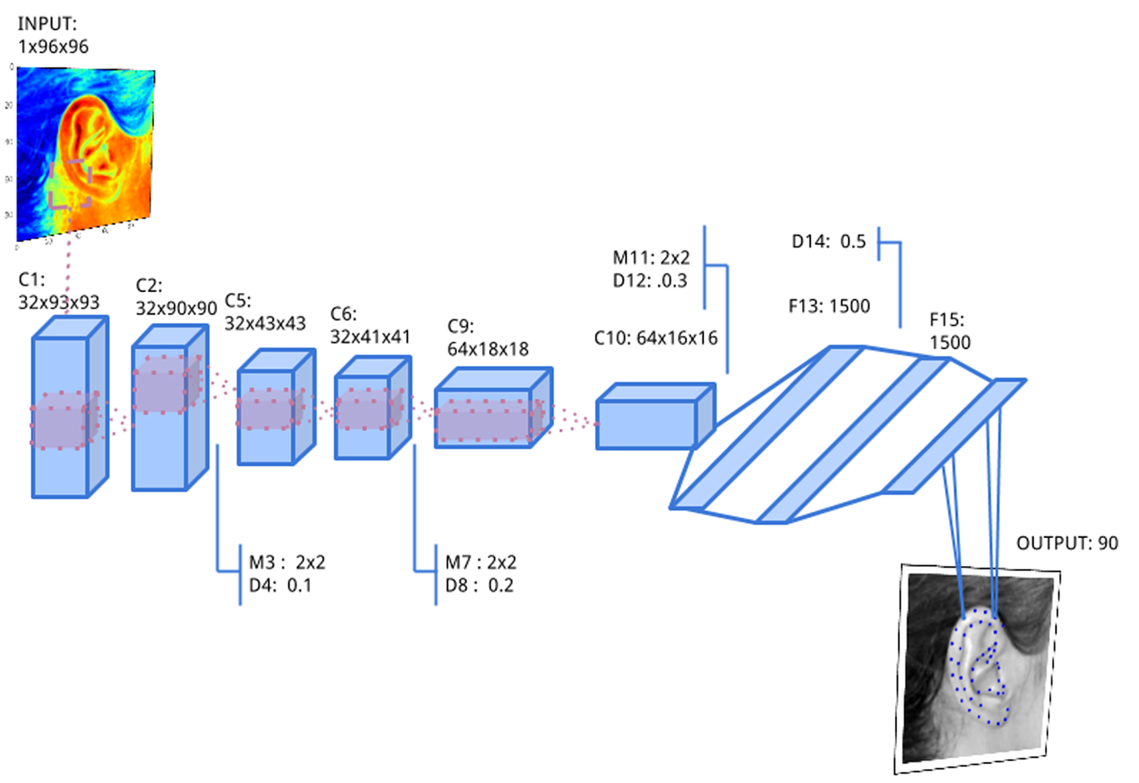
\includegraphics[scale=0.4]{images/ear_cnn}
	\caption{The best architecture for automatic ear's landmarks detection}
	\label{1Econv}
\end{figure}
\subsection{Experiments}
%Following the article, the method is evaluated the usual quality metrics for regression problems, in particular $r^2$, root mean square error (RMSE), explained variance (EV), and Pearson's correlation.
%The accuracy of three architectures are shown in Table \ref{tbear1}. Also, in Table \ref{tbear2}, the RMSE for each landmarks is shown. The regression metrics were computed using \textit{scikit-learn}\cite{}.

%\begin{table}[h!]
%	\centering
%	\begin{tabular}{l c c c}
%	& Arch0 & Arch1 & Arch2 \\ \hline
%	$r^2$ & 0.709 & 0.678 & 0.698 \\ \hline
%	RMSE & 2.296 & 2.415 & 2.338\\ \hline
%	EV & 0.976 & 0.974 &  0.975 \\ \hline
%	Pearson & 0.988 & 0.987 &  0.988 \\ \hline	
%	\end{tabular}
%	\caption{Performance of three different ConvNet architectures}
%	\label{tbear1}
%\end{table}\\
%\begin{table}[h!]
%	\centering
%	\begin{tabular}{l r}
%	\# Landmark & RMSE \\ \hline
%	1 & 1.8183 \\ \hline
%	2 & 1.2216\\ \hline
%	3 &  1.08651\\ \hline
%	4 &  1.3291\\ \hline
%	5 &  2.4477\\ \hline
%	6 &  2.59746\\ \hline
%	7 &  1.17571\\ \hline
%	\end{tabular}
%	\caption{RMS error for each landmark}
%	\label{tbear2}
%\end{table}\\

Because the CANDELA dataset is not published. Another dataset was chosen to study the network. The new dataset was used for the Facial Keypoint Detection including 7049 gray-scale images ($96 \times 96$). For each image, we are supported learn to find the position of 15 landmarks. After dropping some missing data, the dataset remains 2140 images. All the images with coordinates of manual landmarks is stored in csv file and fetched into the network. During the training and validation, the usual quality metrics for regression problems is used, in particular, root mean square error (RMSE). Fig.\ref{earLosstrain} shows the learning curves of the model on training and validation set error. The training is finished after 3000 iterations with the loss arround $10^{-3}$.
\begin{figure}[h!]
	\centering
	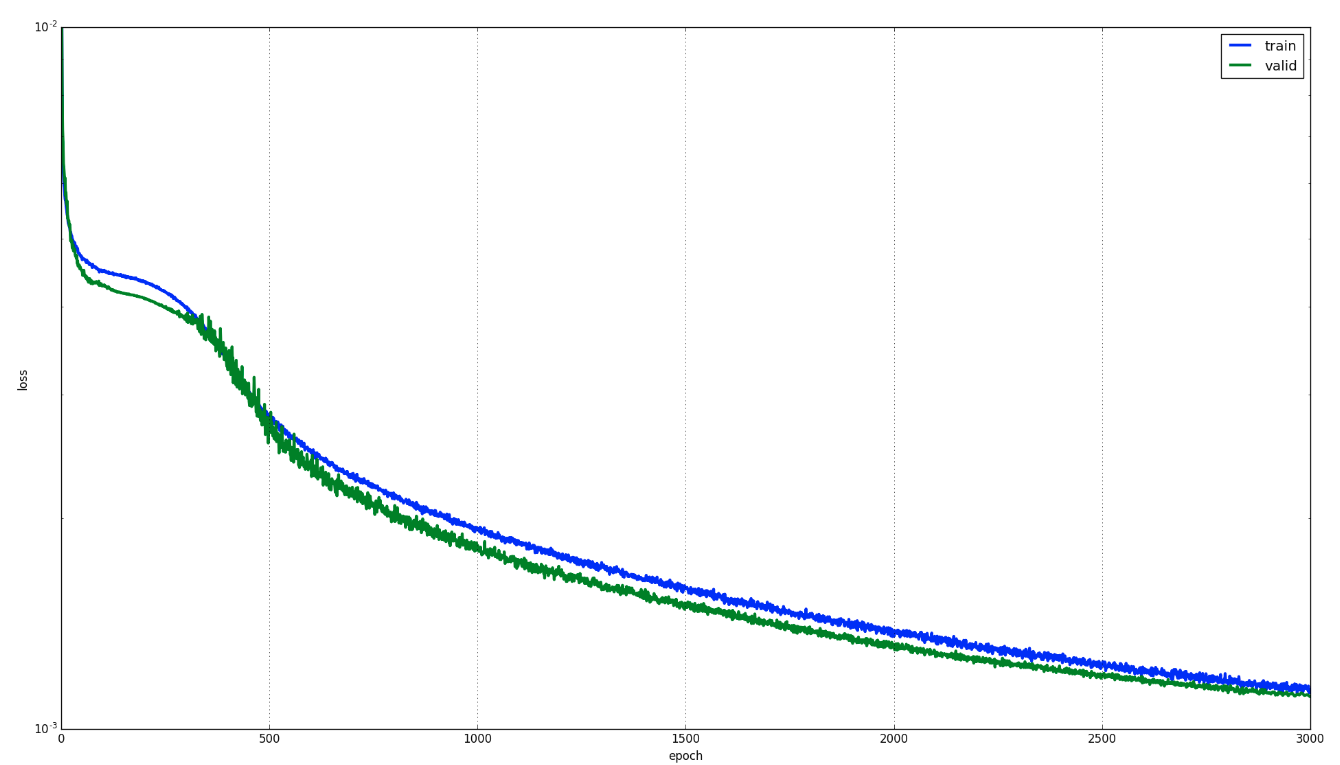
\includegraphics[scale=0.27]{images/trainloss}
	\caption{The loss of Ear-CNN network on facial point dataset}
	\label{earLosstrain}
\end{figure}
Fig.\ref{earTest} shows some test on the real facial images.
\begin{figure}[h!]
	\centering
	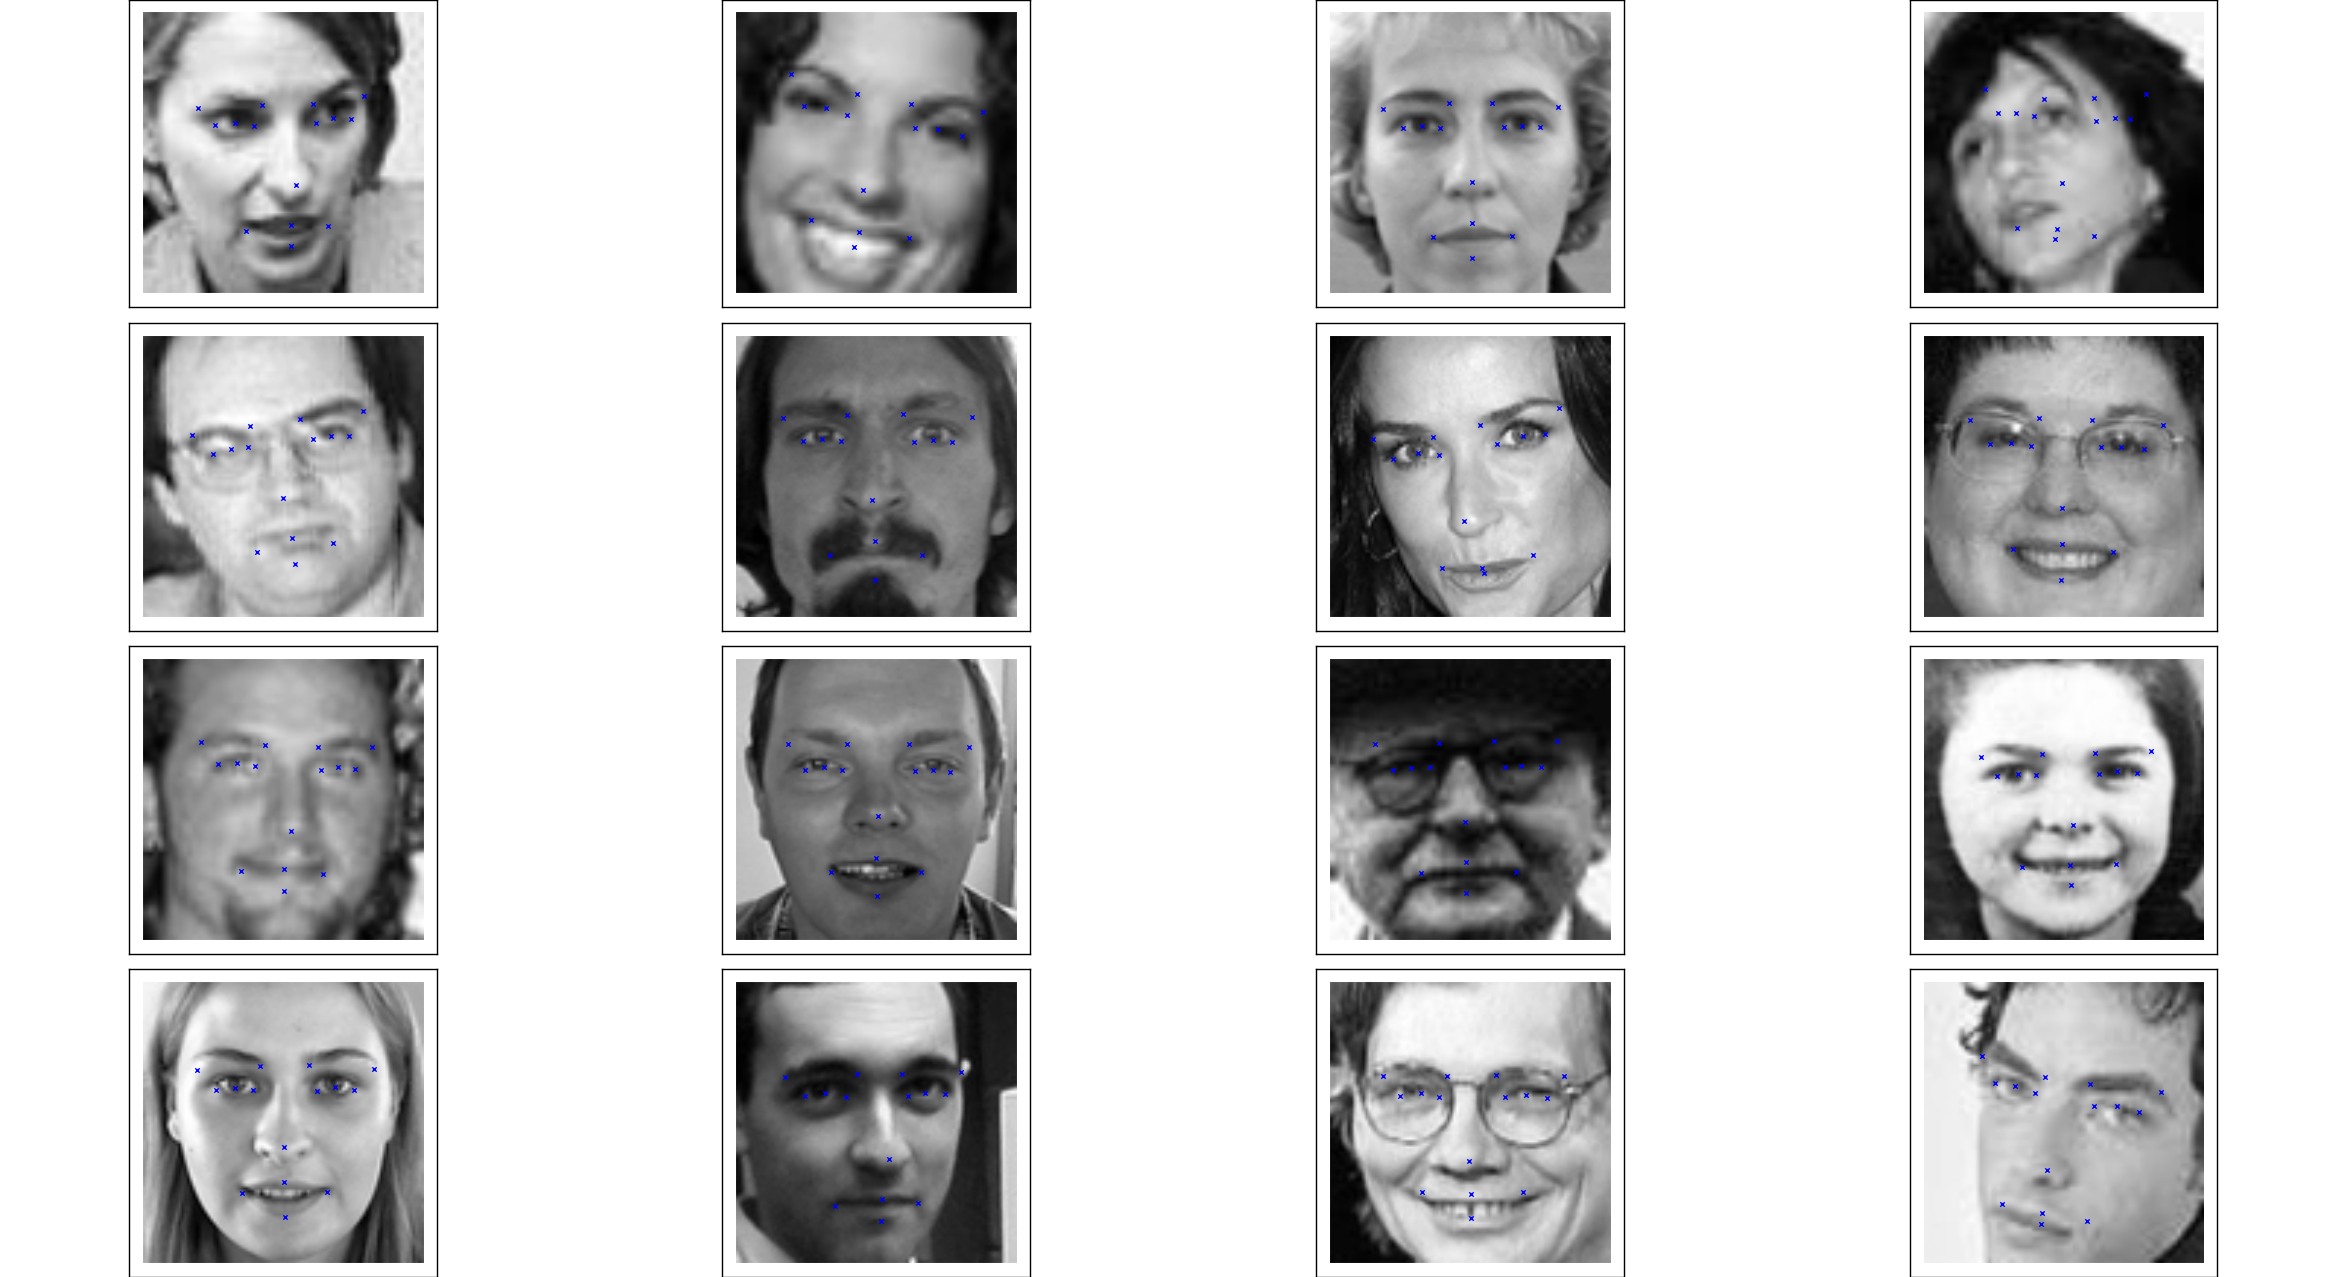
\includegraphics[scale=0.27]{images/figure_1-1.png}
	\caption{The prediction landmarks on human face}
	\label{earTest}
\end{figure}
\section{Model 1 and model 2 on pronotum}
\subsection{Dataset preparing}
The dataset includes 293 pronotum images. The images are divided into three subsets: the training set (200 images), the validation set (60 images) and the testing set (33 images). Because the dataset is limited and the models are worked on gray-scale images, we applied some ways to en-large the dataset. Firstly, for each original image in RGB, each channel is modified by adding some values. Secondly, the channels of the original image are split. So, we have obtained 1400 images for the training set and 420 images for the validation set. At the end, the images are down-sampled with the  size of $256 \times 192$ before giving to the networks.

%To enlarge the dataset during training, the image in training and validation set are augmentation by modifying the valued of red and green channel. So, at the end, we have 600 and 180 images in training and validation set, respectively.
\subsection{Model 1 and pronotum landmarks}
The networks in the first level are modified to suitable with the prediction of landmarks on the pronotum (8-landmarks). For each pronotum, eight manual landmarks have been set. The bounding box is created depending on the coordinate of the manual landmark and kept with the same size. The networks in the first level are used as followed:
\begin{itemize}
	\item F1 network recognizes whole pronotum bounding box with eight landmarks.
	\item EN1 network predicts the location of the first five-landmarks i.e $[1..5]$.
	\item NM1 network is used to estimated the position of last four-landmarks and the first landmark i.e $[5..8,1]$.
	\item At the end, the position of each landmark is average of the predicted position in the networks.
\end{itemize} 
\subsubsection{Testing}
During training, the Euclidean distance (sum of squares) is used to compute the loss of the networks. The error rate of each network during training is shown in the Table.\ref{model1p}:\\
\begin{table}[h!]
	\centering
	\begin{tabular}{l r}
	Network & Loss \\ \hline
	F1 & 0.013 \\ \hline
	EN1 & 0.47\\ \hline
	NM1 &  0.5
	\end{tabular}
	\caption{The loss of the networks in Model 1 on pronotum dataset}
	\label{model1p}
\end{table}
\begin{figure}[h!]
\centering
\subfloat[Test 1]{\label{}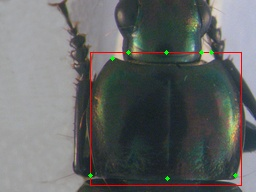
\includegraphics[width=0.2\textwidth]{./images/test1}}~~
\subfloat[Test 2]{\label{}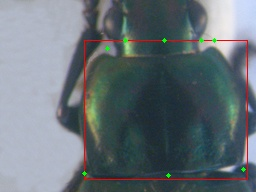
\includegraphics[width=0.2\textwidth]{./images/test2}}\\
\subfloat[Test 3]{\label{}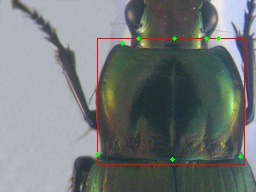
\includegraphics[width=0.2\textwidth]{./images/test3}}~~
\subfloat[Test 4]{\label{}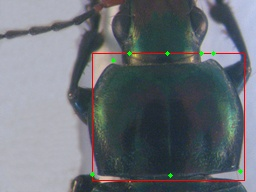
\includegraphics[width=0.2\textwidth]{./images/test4}}\\
\caption{The pronotum with predicted landmarks at level 1}
\label{model1pTest}
\end{figure}\\
From Table \ref{model1p}, the errors of EN1 and NM1 are still high. That errors make the prediction result of level 1 do not enough good. Besides, the networks at level 2 and level 3 used the prediction at level 1 as the input data to predict the new position. So, we can not continue with the level 2, 3 until the result at level 1 is improved. Perhaps, the model in model 1 is not suitable to detect the landmarks on pronotum.  Fig. \ref{model1pTest} shows the prediction landmarks on four images. Followed that, the networks can detect the landmarks at positions 4, 5 and 7; the different positions still not good.
\subsection{Model 2 and pronotum landmarks}
The dataset is kept the same with model 1 (1400 images for training and 420 images for validation) but having some changes. Firstly, the ways to choose the data(to train and validate) is changed. All images are combined. Then, the network will automatically choose $75 \%$ data to train and $25 \%$ for validation. Secondly, the inputs that given to the network are just the image and landmarks(without the coordinates of the bounding box).

The network is run 3000 iterations with the learning rate begin from $0.08$ to $0.01$. During training, the learning rate is changed to fit with the remaining iterations\cite{lecun2012efficient}. Fig.\ref{model2pl} shows the first 700 iterations during training. The loss did not have many changes after $100^{th}$ iteration.

\begin{figure}[h!]
	\centering
	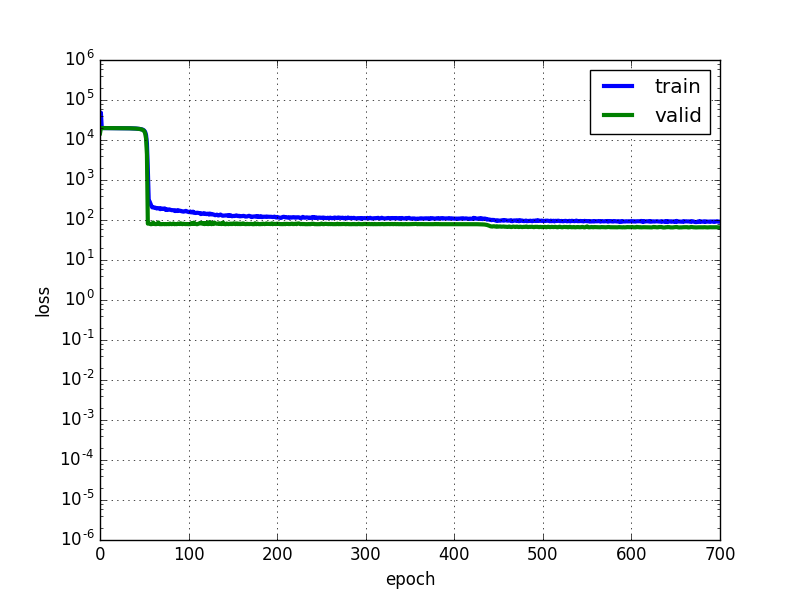
\includegraphics[scale=0.4]{images/figure_1_loss_celia}
	\caption{The losses of model 2 on pronotum dataset}
	\label{model2pl}
\end{figure}

\begin{figure}[h!]
	\centering
	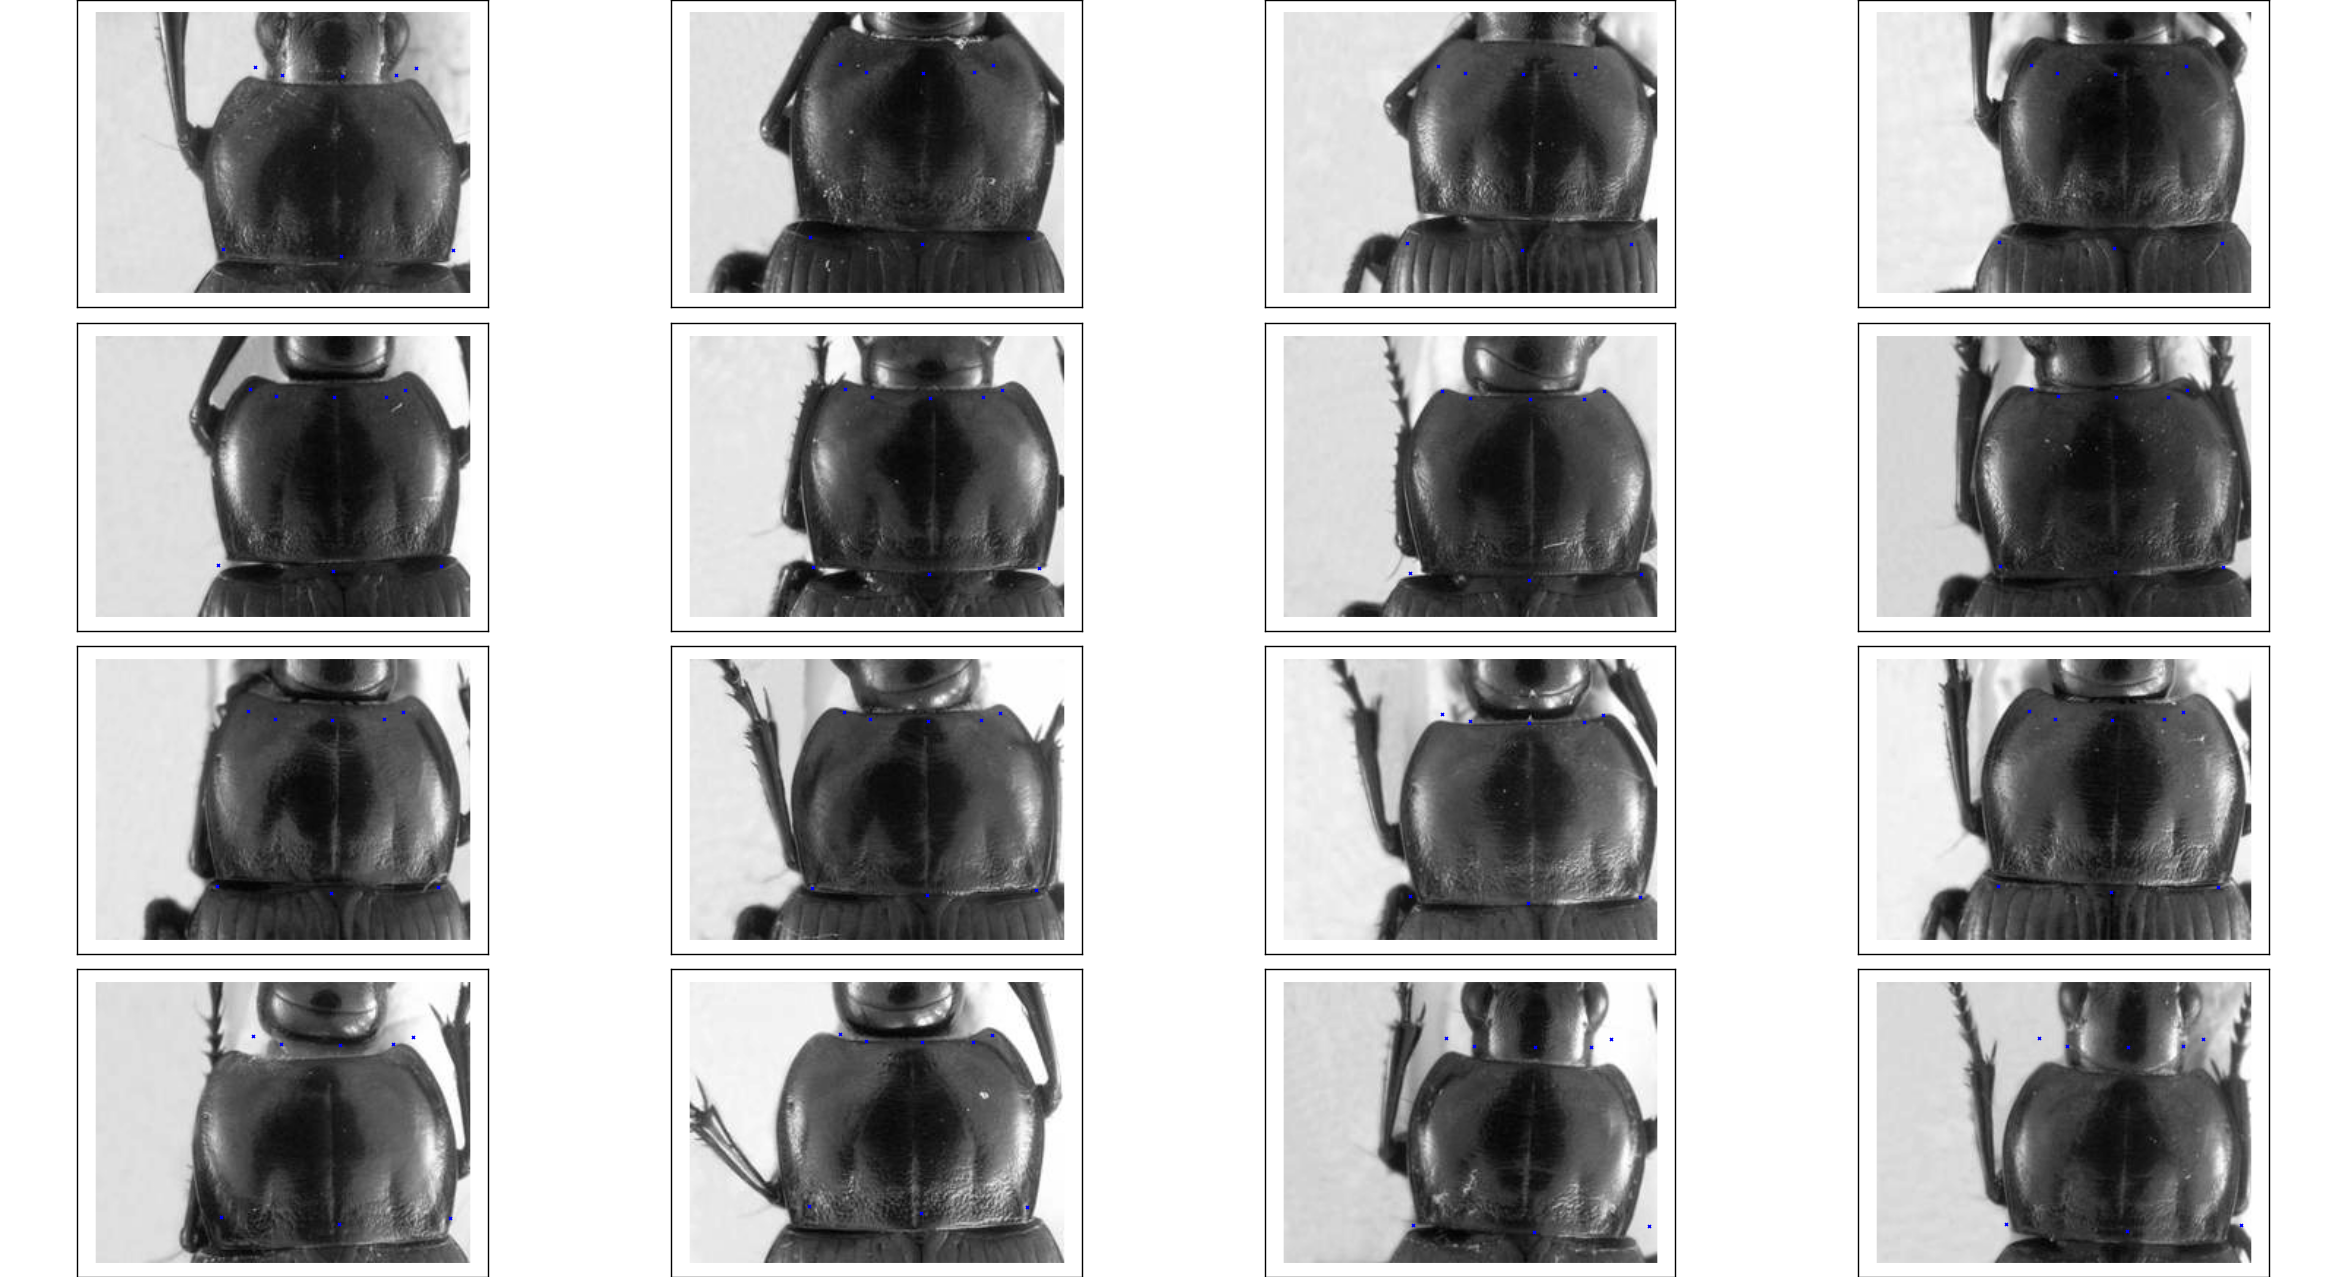
\includegraphics[scale=0.25]{images/figure_1_celia}
	\caption{The prediction landmarks on pronotum of model 2}
	\label{model2pt}
\end{figure}
Fig.\ref{model2pt} shows the prediction landmarks on 16 images. Following, the prediction landmarks from the network of model 2 are closed with the pronotum but the location is still inaccurate.

%\subsection{Comparing model 1 and model 2}
%Table C shows some differences from 2 models
%\begin{table}[h!]
%	\centering
%	\begin{tabular}{l c c c}
%	Model & Framework & Dataset (images) & Learning rate \\ \hline
%	Model 1 & Caffe & 13466 & 0.013 \\ \hline
%	Model 2 & Lasagne(Theano) & 2140 & zz\\
%	\end{tabular}
%\end{table}\\
\section{Proposed architecture (model 3)}
\subsection{Model and parameters}
From the tutorial of Daniel Nouri\footnote{http://danielnouri.org/} about using CNN to detect facial key points. We propose a CNN to detect the landmarks on pronotum. The proposed network includes three convolutional layers followed by three maximum pooling layers and three full connected layers(Fig.\ref{pmodel}). The network receives the gray-scale image ($256 \times 192$) as the input. The deep of convolutional layers is increased from $32, 64, $ to $ 128$ with different size of filter. The size of filters in pooling layers are kept in the same size of $2 \times 2$. At the end of network, three full-connected layers with the size of $500, 500, $ and $16$ are set up to predict the positions of landmarks. Besides, the model is designed with a small sharing learning-rate and the momentum. The learning-rate and the momentum are changed overtime of training.
\begin{figure}[h!]
	\centering
	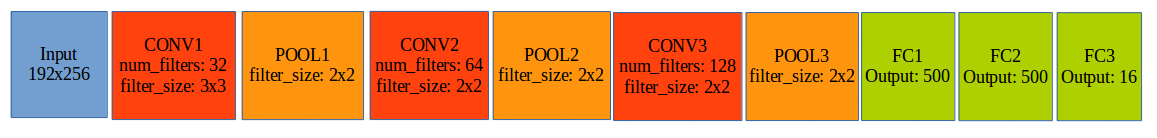
\includegraphics[scale=0.4]{images/model3}
	\caption{The architecture of proposed model}
	\label{pmodel}
\end{figure}
\subsection{Training and experiments}
The model is trained with 1820 images in 5000 iterations. The images are normalized before giving to the network by scaling the intensity value to [0,1], instead of 0 to 255. The target values (x and y coordinates) is kept as original. During the training, the root-mean-square error (MSE) is used to calculate the loss.

To evaluate the stability and confidence of the model, we proposed several rules to select the images for the network, as Table.\ref{choosedata}:\\
\begin{table}[h!]
	\centering
	\begin{tabular}{c l l}
	Rule & Test set & Training and validation set \\ \hline
	rule\_1 & From $1^{st}$ image to $33^{rd}$ image & Remaining images \\ \hline
	rule\_2 & From $260^{th}$ image to $293^{rd}$ image & Remaining images\\ \hline
	rule\_3 & Random & Random \\ \hline
	rule\_4 & From $90^{th}$ image to $122^{nd}$ image & Remaining images\\ \hline
	rule\_5 & From $200^{th}$ image to $232^{nd}$ image & Remaining images \\ \hline
	\end{tabular}
	\caption{The rules to choose the data for the network}
	\label{choosedata}
\end{table}~\\
Following the rules to choose the data, the loss of training and validation is shown in Table \ref{losschoosedata}. From the results in the table, the training losses in the cases of \textit{rule\_4, rule\_5} are smaller than other rules; but the validation losses are stability. It means the overfitting is appeared clearly in the case of \textit{rule\_4} and \textit{rule\_5}. In which, the smallest difference value between training and validation loss is belong to \textbf{random} case.
\begin{table}[h!]
	\centering
	\begin{tabular}{c l l}
	Rule & Training loss & Validation loss \\ \hline
	rule\_1 & $0.12739$ & $0.63681$ \\ \hline
	rule\_2 & $0.15204$ & $0.59480$ \\ \hline
	rule\_3 & $0.16694$ & $0.55584$ \\ \hline
	rule\_4 & $0.08798$ & $0.61934$ \\ \hline
	rule\_5 & $0.0918$ & $0.52843$ \\ \hline
	\end{tabular}
	\caption{The training loss and validation loss following each rule to choose the data}
	\label{losschoosedata}
\end{table}~\\[0.1cm]
Fig.\ref{cnn3l} shows the training curve loss and validation curve loss of the model on each rule to choose the data. From the beginning, the loss is not changed. When the training is longer and the learning rate is improved, the loss is decreased and a large distance between training and validation is appeared (over-fitting) but it is not that bad.

The model is tested on the test datasets(five rules). Then, correlation between the manual landmarks and predicted landmarks is computed by applying the correlation methods (see Table.\ref{pearson}, \ref{spearman}, \ref{kendall})
\begin{table}[h!]
	\centering
	\begin{tabular}{c c c}
		Rule & x correlation & y correlation \\ \hline
		rule\_1 & $0.9953877$ & $0.9941767$ \\ \hline
		rule\_2 & $0.9968787$ & $0.9960827$ \\ \hline
		rule\_3 & $0.9966784$ & $0.9957729$ \\ \hline
		rule\_4 & $0.9975662$ & $0.9985097$ \\ \hline
		rule\_5 & $0.9972048$ & $0.9976416$ \\ \hline
	\end{tabular}
	\caption{The correlation between manual and predicted landmarks by Pearson\cite{pallant2013spss} method}
	\label{pearson}
\end{table}
\begin{table}[h!]
	\centering
	\begin{tabular}{c c c}
		Rule & x correlation & y correlation \\ \hline
		rule\_1 & $0.9893943$ & $0.9289319$ \\ \hline
		rule\_2 & $0.992556$ & $0.9444423$ \\ \hline
		rule\_3 & $0.9913126$ & $0.9565425$ \\ \hline
		rule\_4 & $0.9943106$ & $0.9789221$ \\ \hline
		rule\_5 & $0.9920646$ & $0.9864683$ \\ \hline
	\end{tabular}
	\caption{The correlation between manual and predicted landmarks by Spearman\cite{myers2010research} method}
	\label{spearman}
\end{table}
\begin{table}[h!]
	\centering
	\begin{tabular}{c c c}
		Rule & x correlation & y correlation \\ \hline
		rule\_1 & $0.913517$ & $0.7498531$ \\ \hline
		rule\_2 & $0.9303295$ & $0.8231899$ \\ \hline
		rule\_3 & $0.9273002$ & $0.8273057$ \\ \hline
		rule\_4 & $0.9419902$ & $0.8904413$ \\ \hline
		rule\_5 & $0.9299128$ & $0.9051508$ \\ \hline
	\end{tabular}
	\caption{The correlation between manual and predicted landmarks by Kendall\cite{kendall1938new} method}
	\label{kendall}
\end{table}

\begin{figure}[h!]
\centering
\subfloat[rule\_1]{\label{}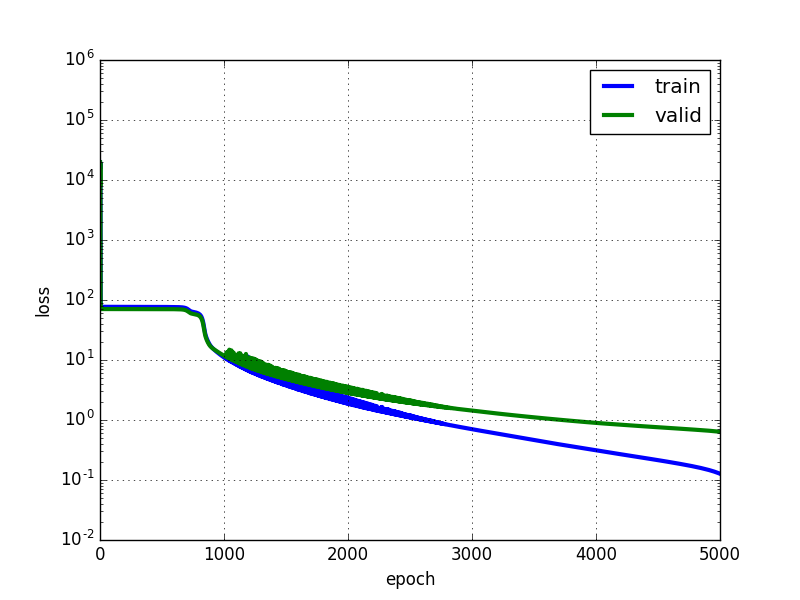
\includegraphics[width=0.4\textwidth]{./images/figure_1_cnn3_5000_loss_v11}}~~
\subfloat[rule\_2]{\label{}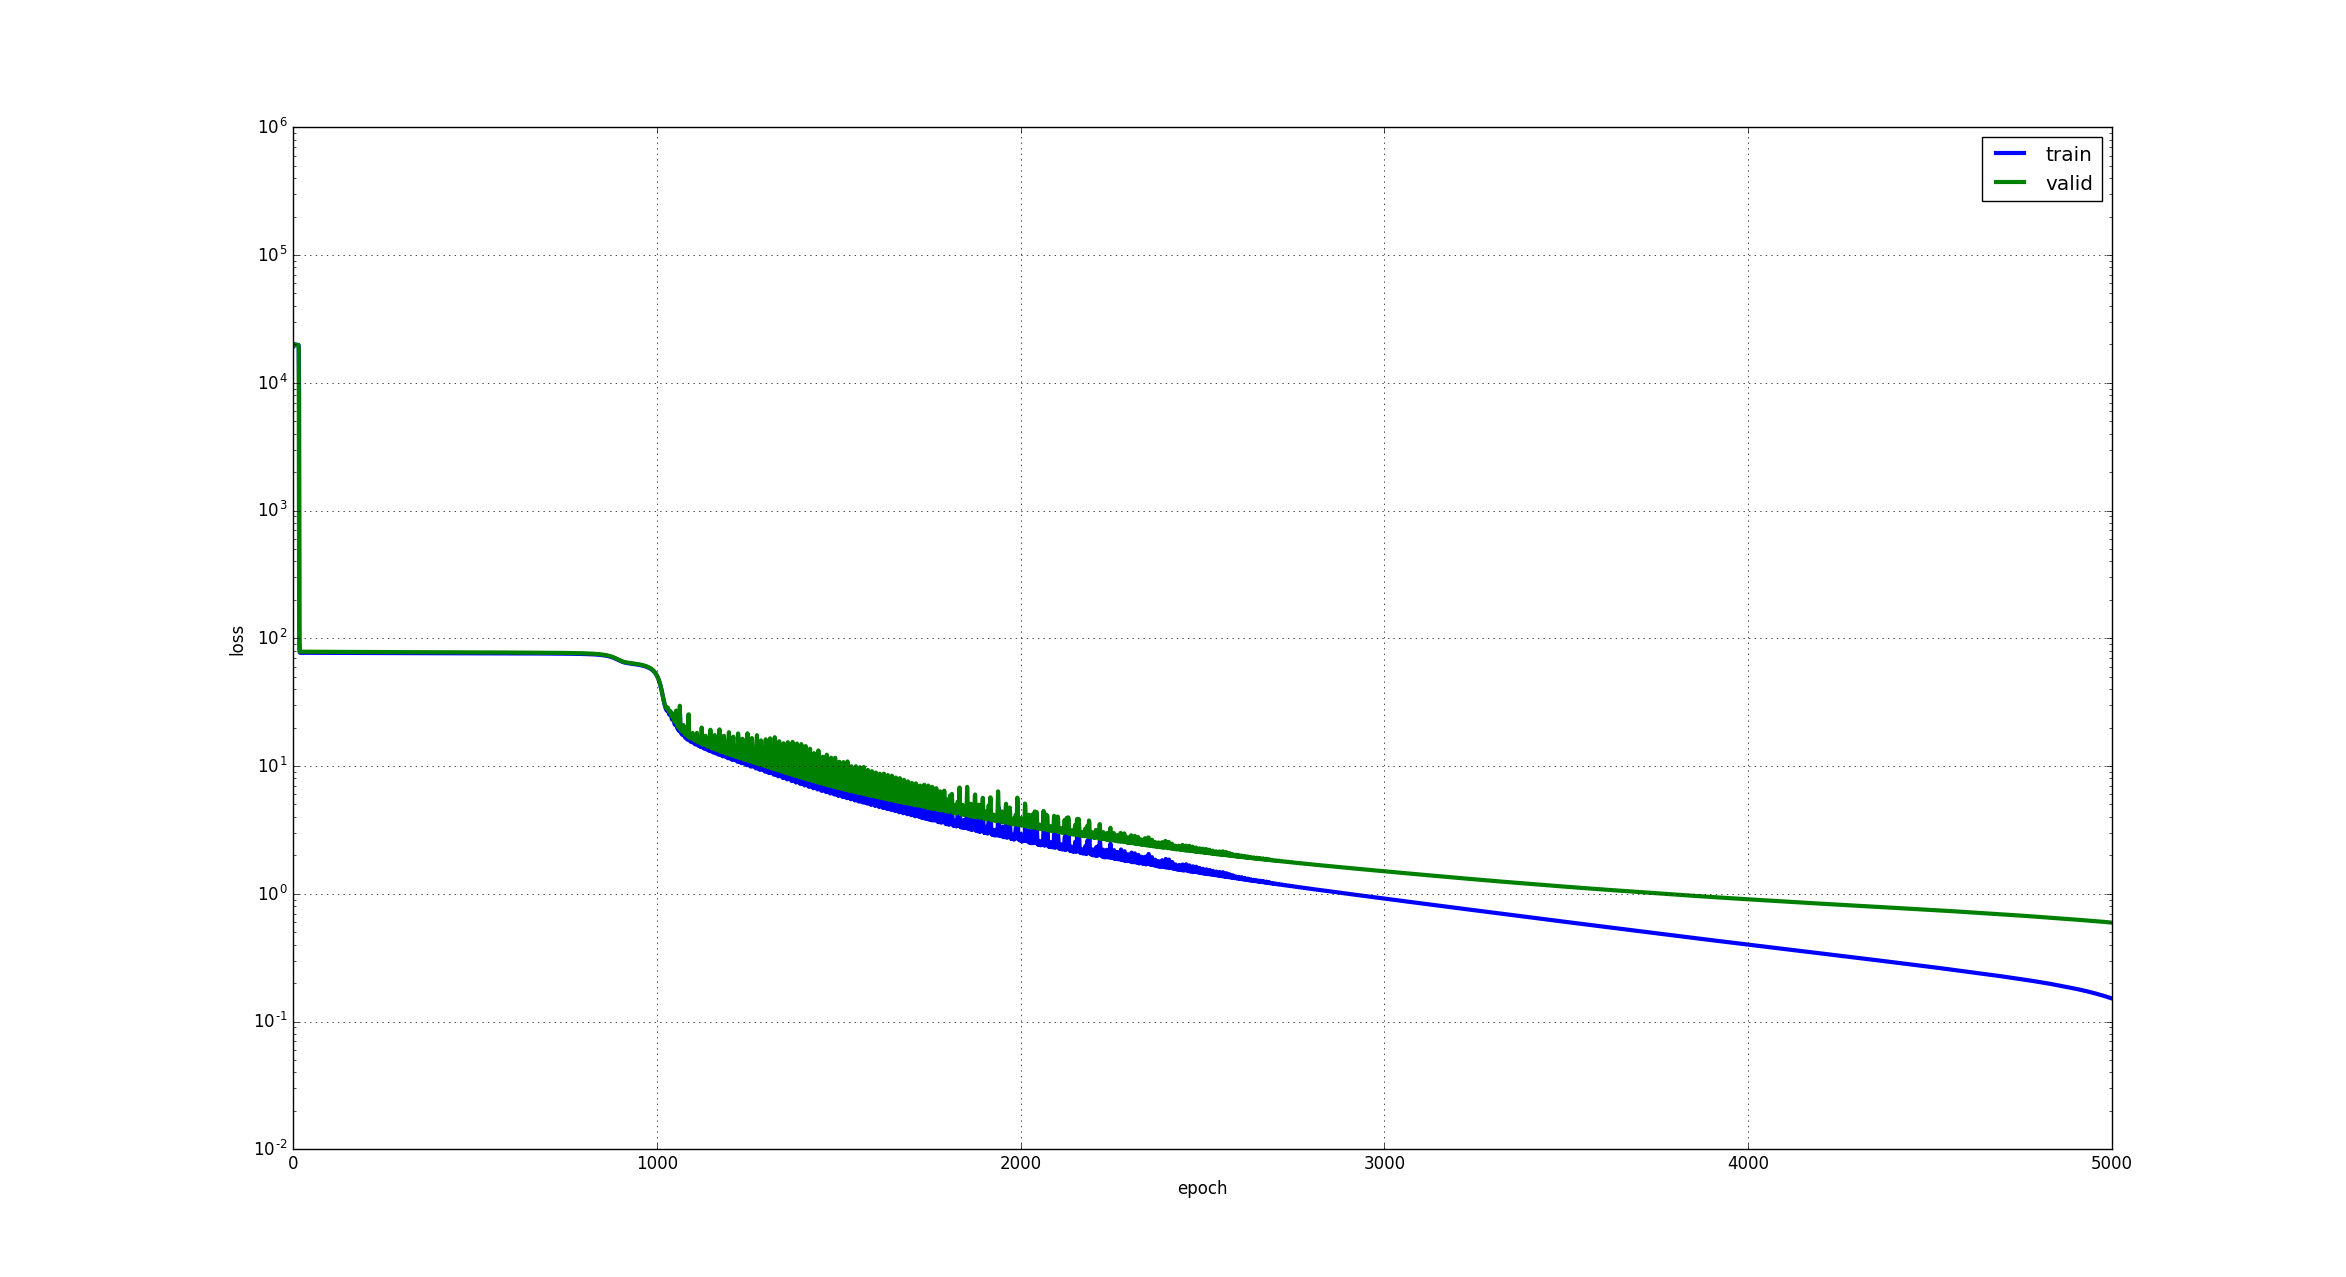
\includegraphics[width=0.4\textwidth]{./images/figure_1_cnn3_5000_loss_v12}}\\
\subfloat[rule\_3]{\label{}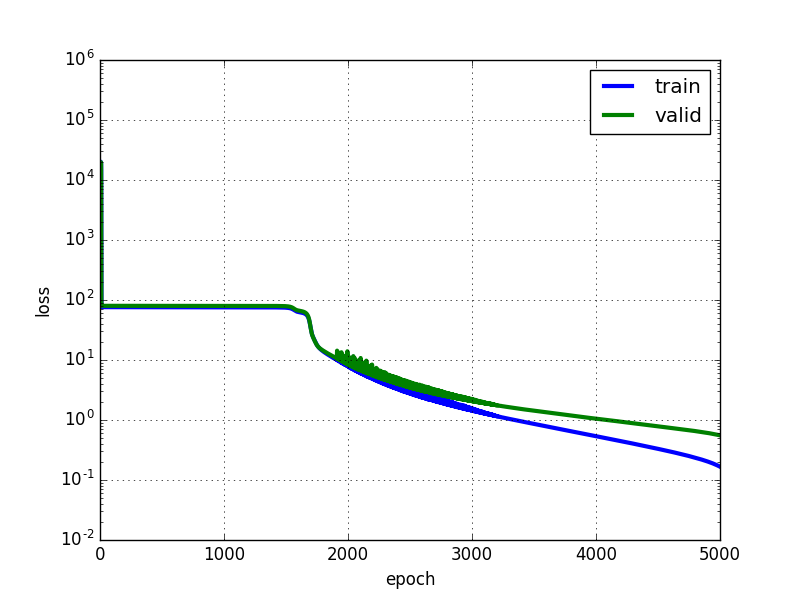
\includegraphics[width=0.4\textwidth]{./images/figure_1_cnn3_5000_loss_v13}}\\
\subfloat[rule\_4]{\label{}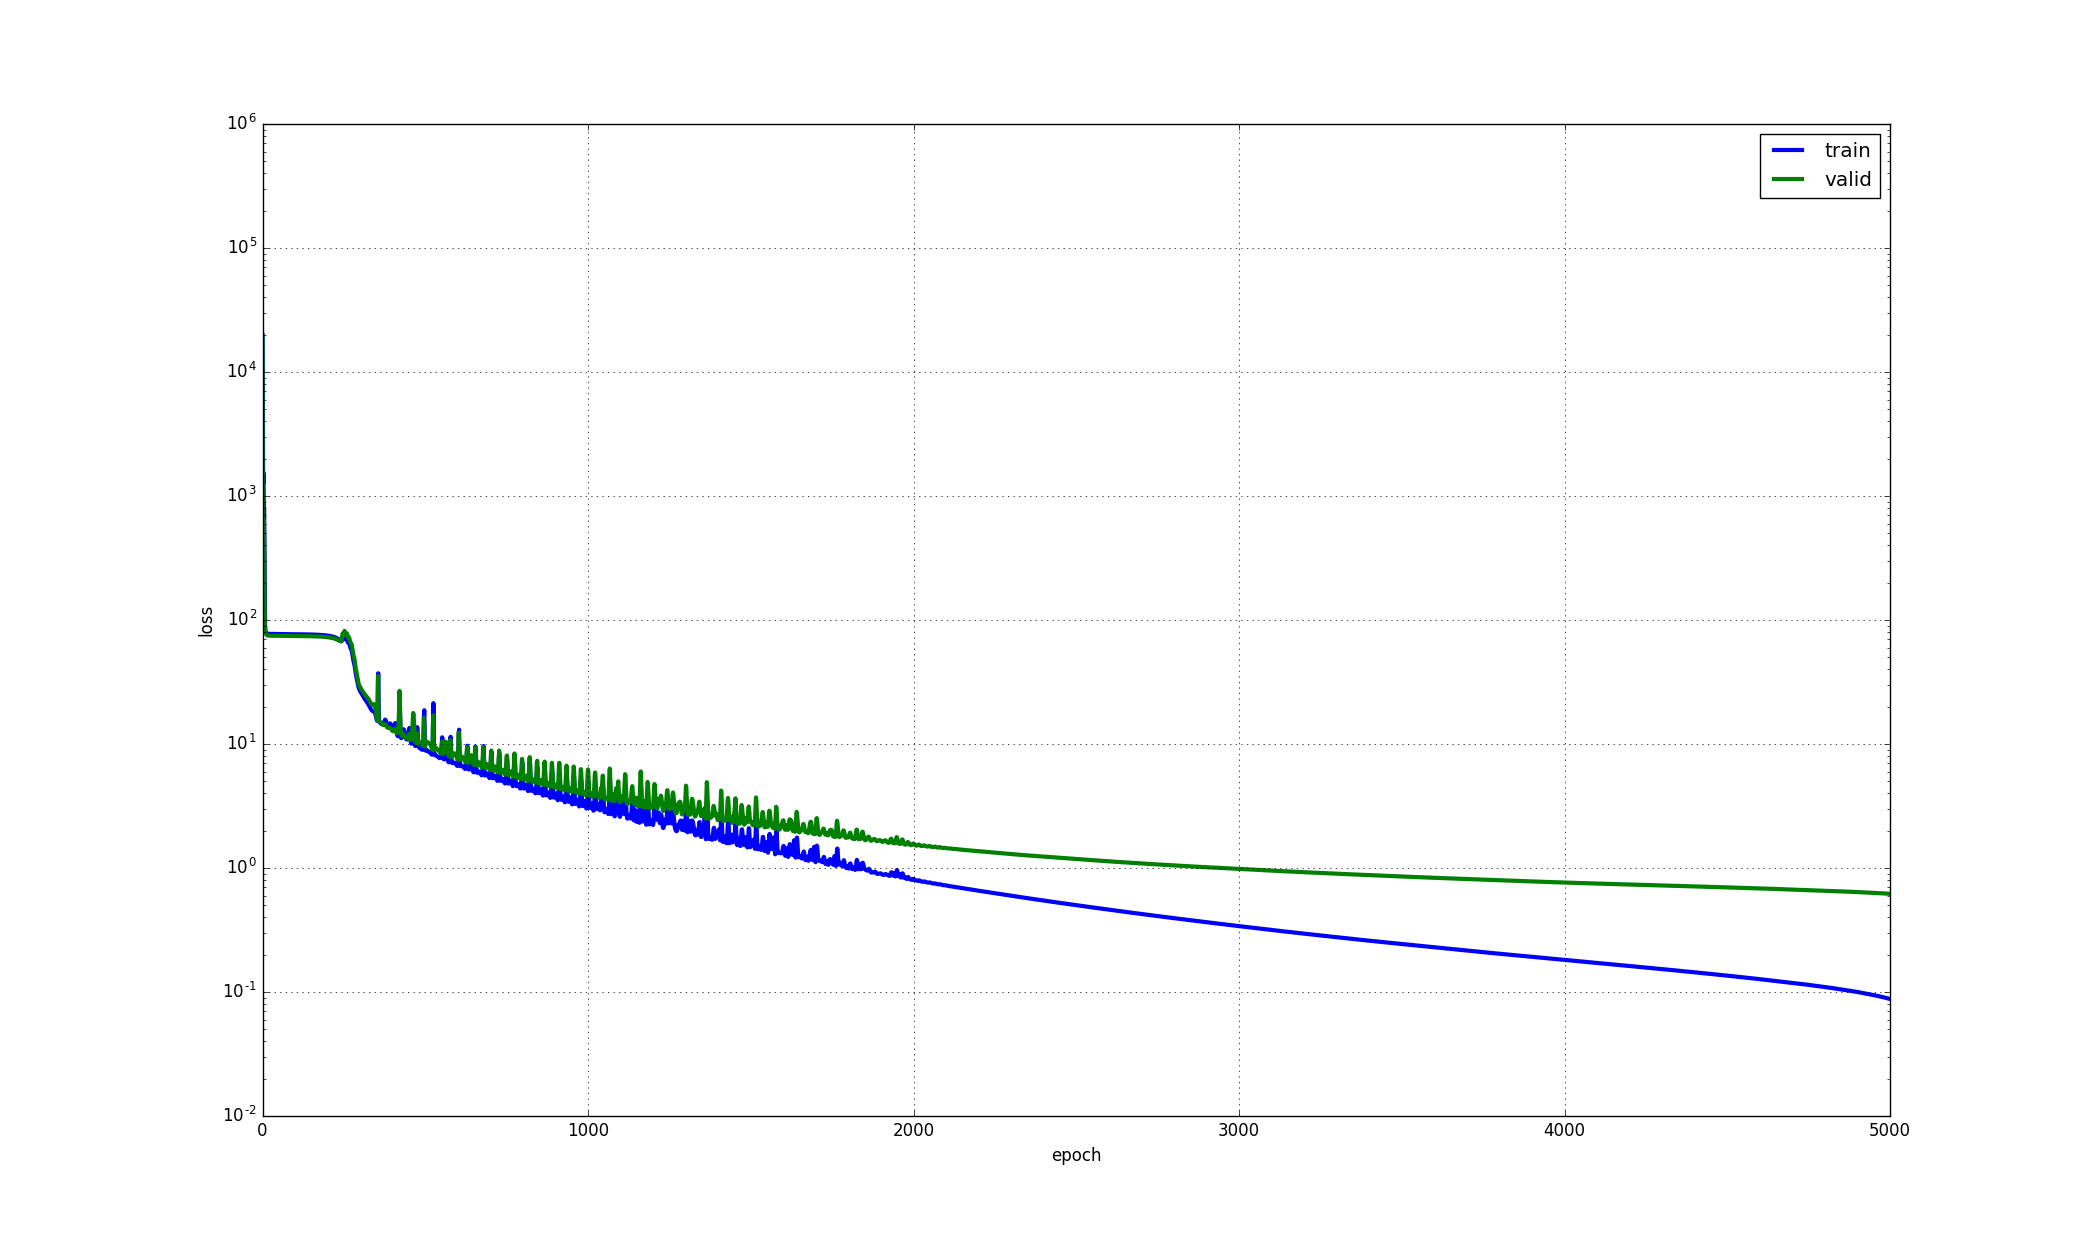
\includegraphics[width=0.4\textwidth]{./images/figure_1_cnn3_5000_loss_v14}}~~
\subfloat[rule\_5]{\label{}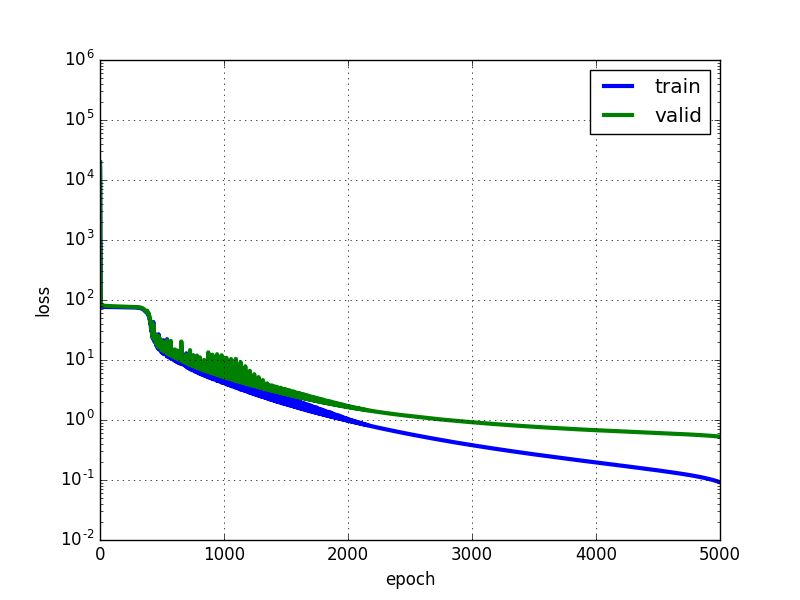
\includegraphics[width=0.4\textwidth]{./images/figure_1_cnn3_5000_loss_v15}}
\caption{The loss during training and validation followed each rule to choose data }
\label{cnn3l}
\end{figure}
\pagebreak

Fig.\ref{cnn3t} show the predicted positions on test dataset followed rule\_3:
%\begin{figure}[h!]
%	\centering
%	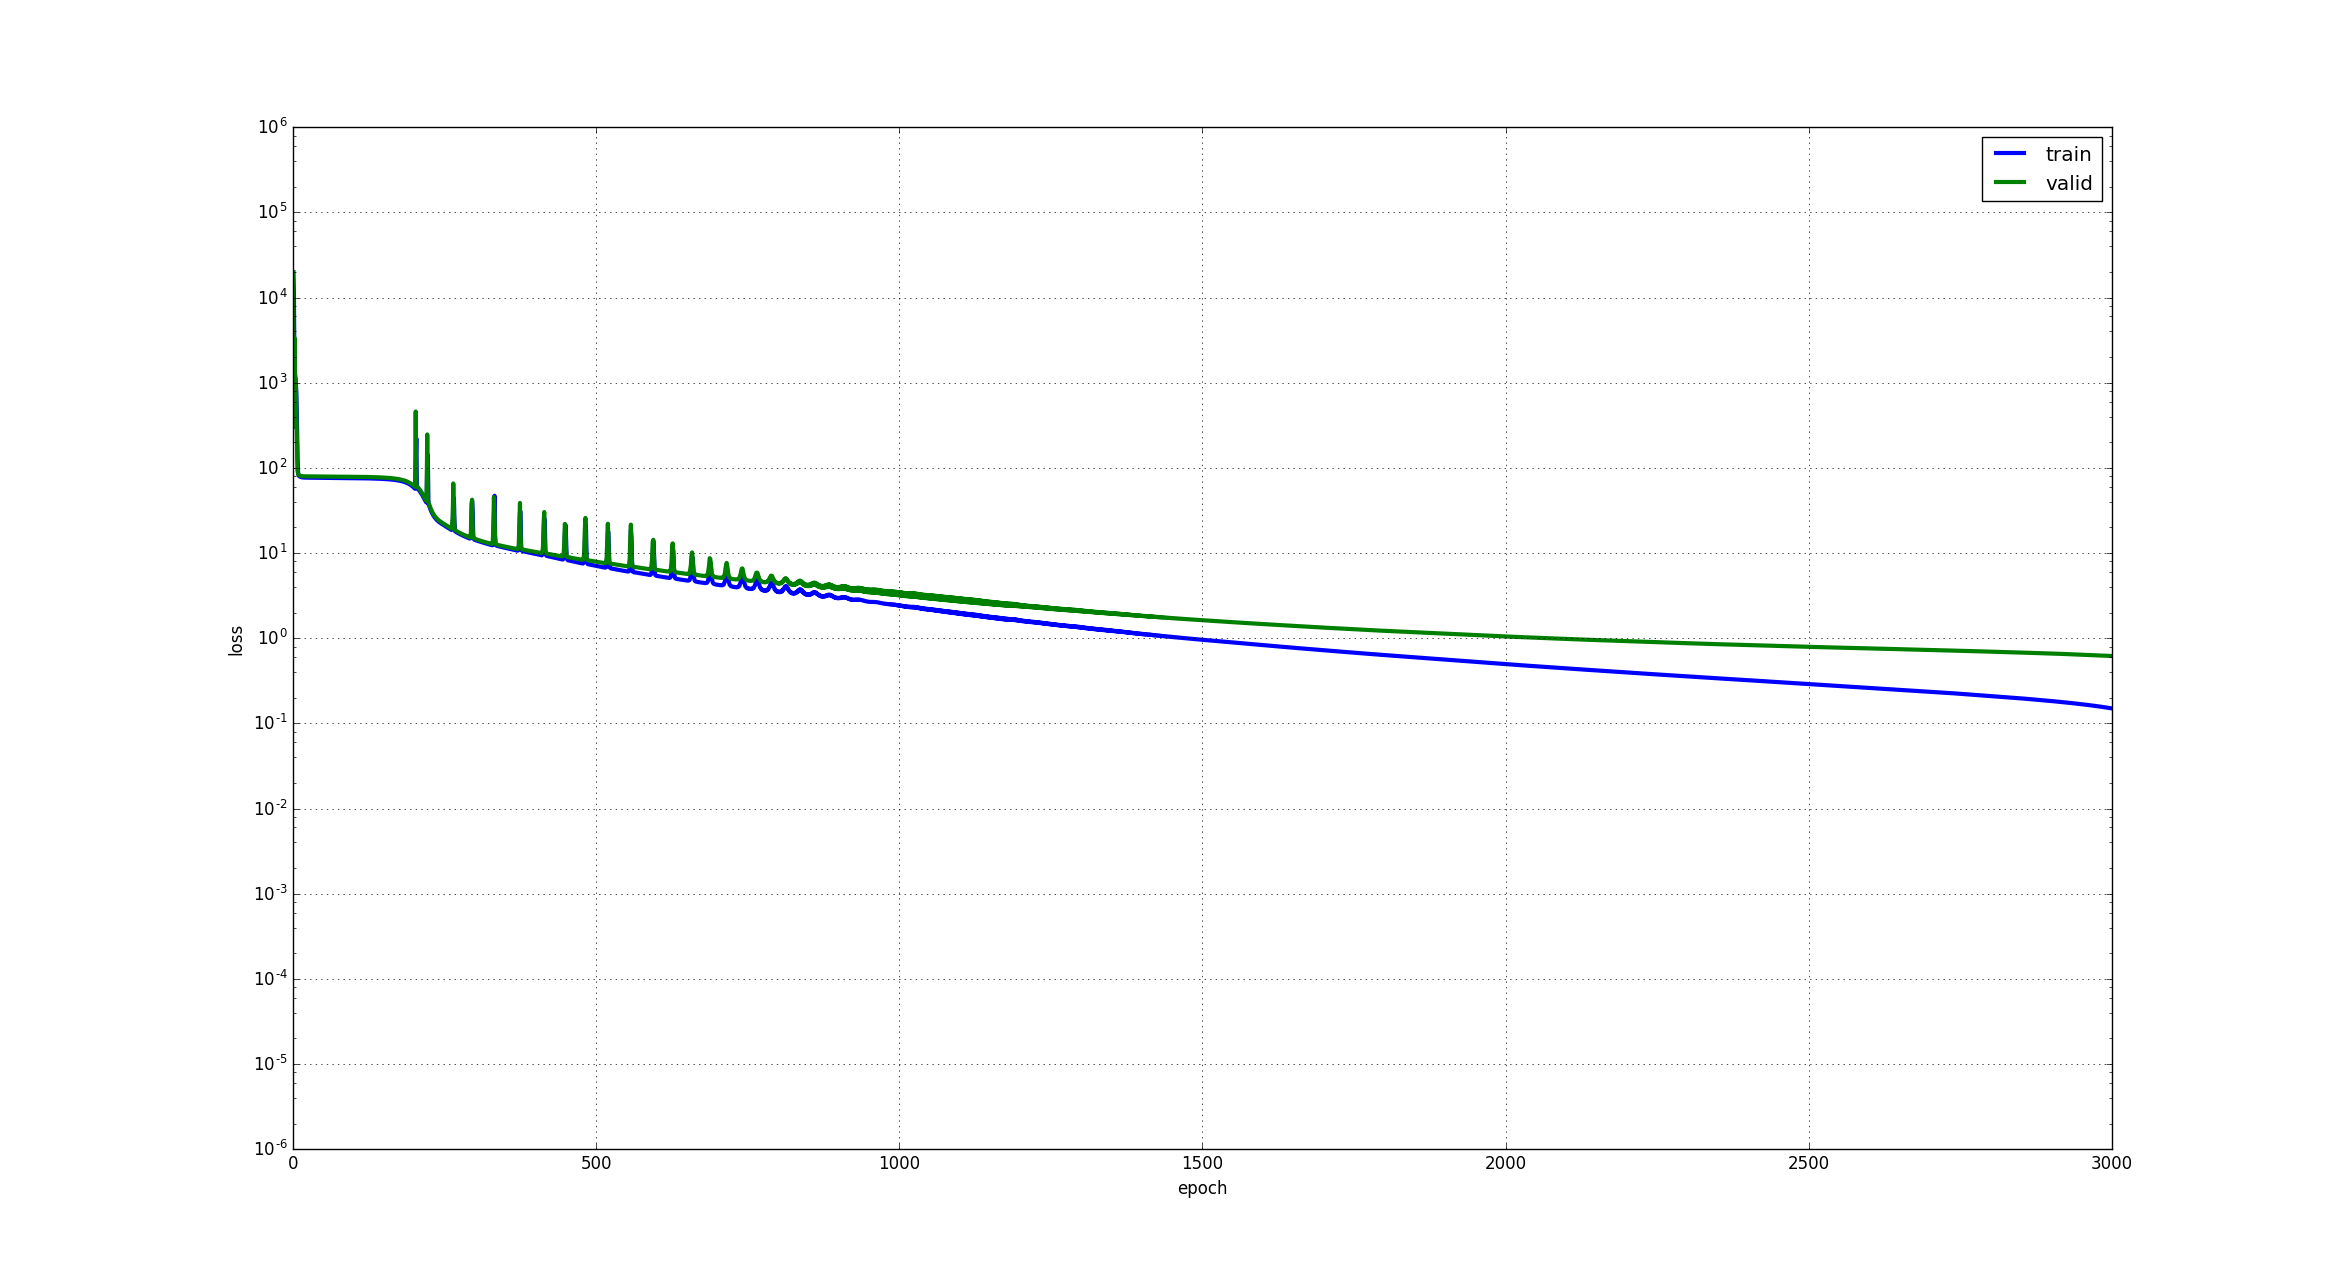
\includegraphics[scale=0.2]{images/figure_1_loss_cnn3_3000_2}
%	\caption{The loss during training and validation of rule\_1}
%	\label{cnn3l}
%\end{figure}
\begin{figure}[h!]
	\centering
	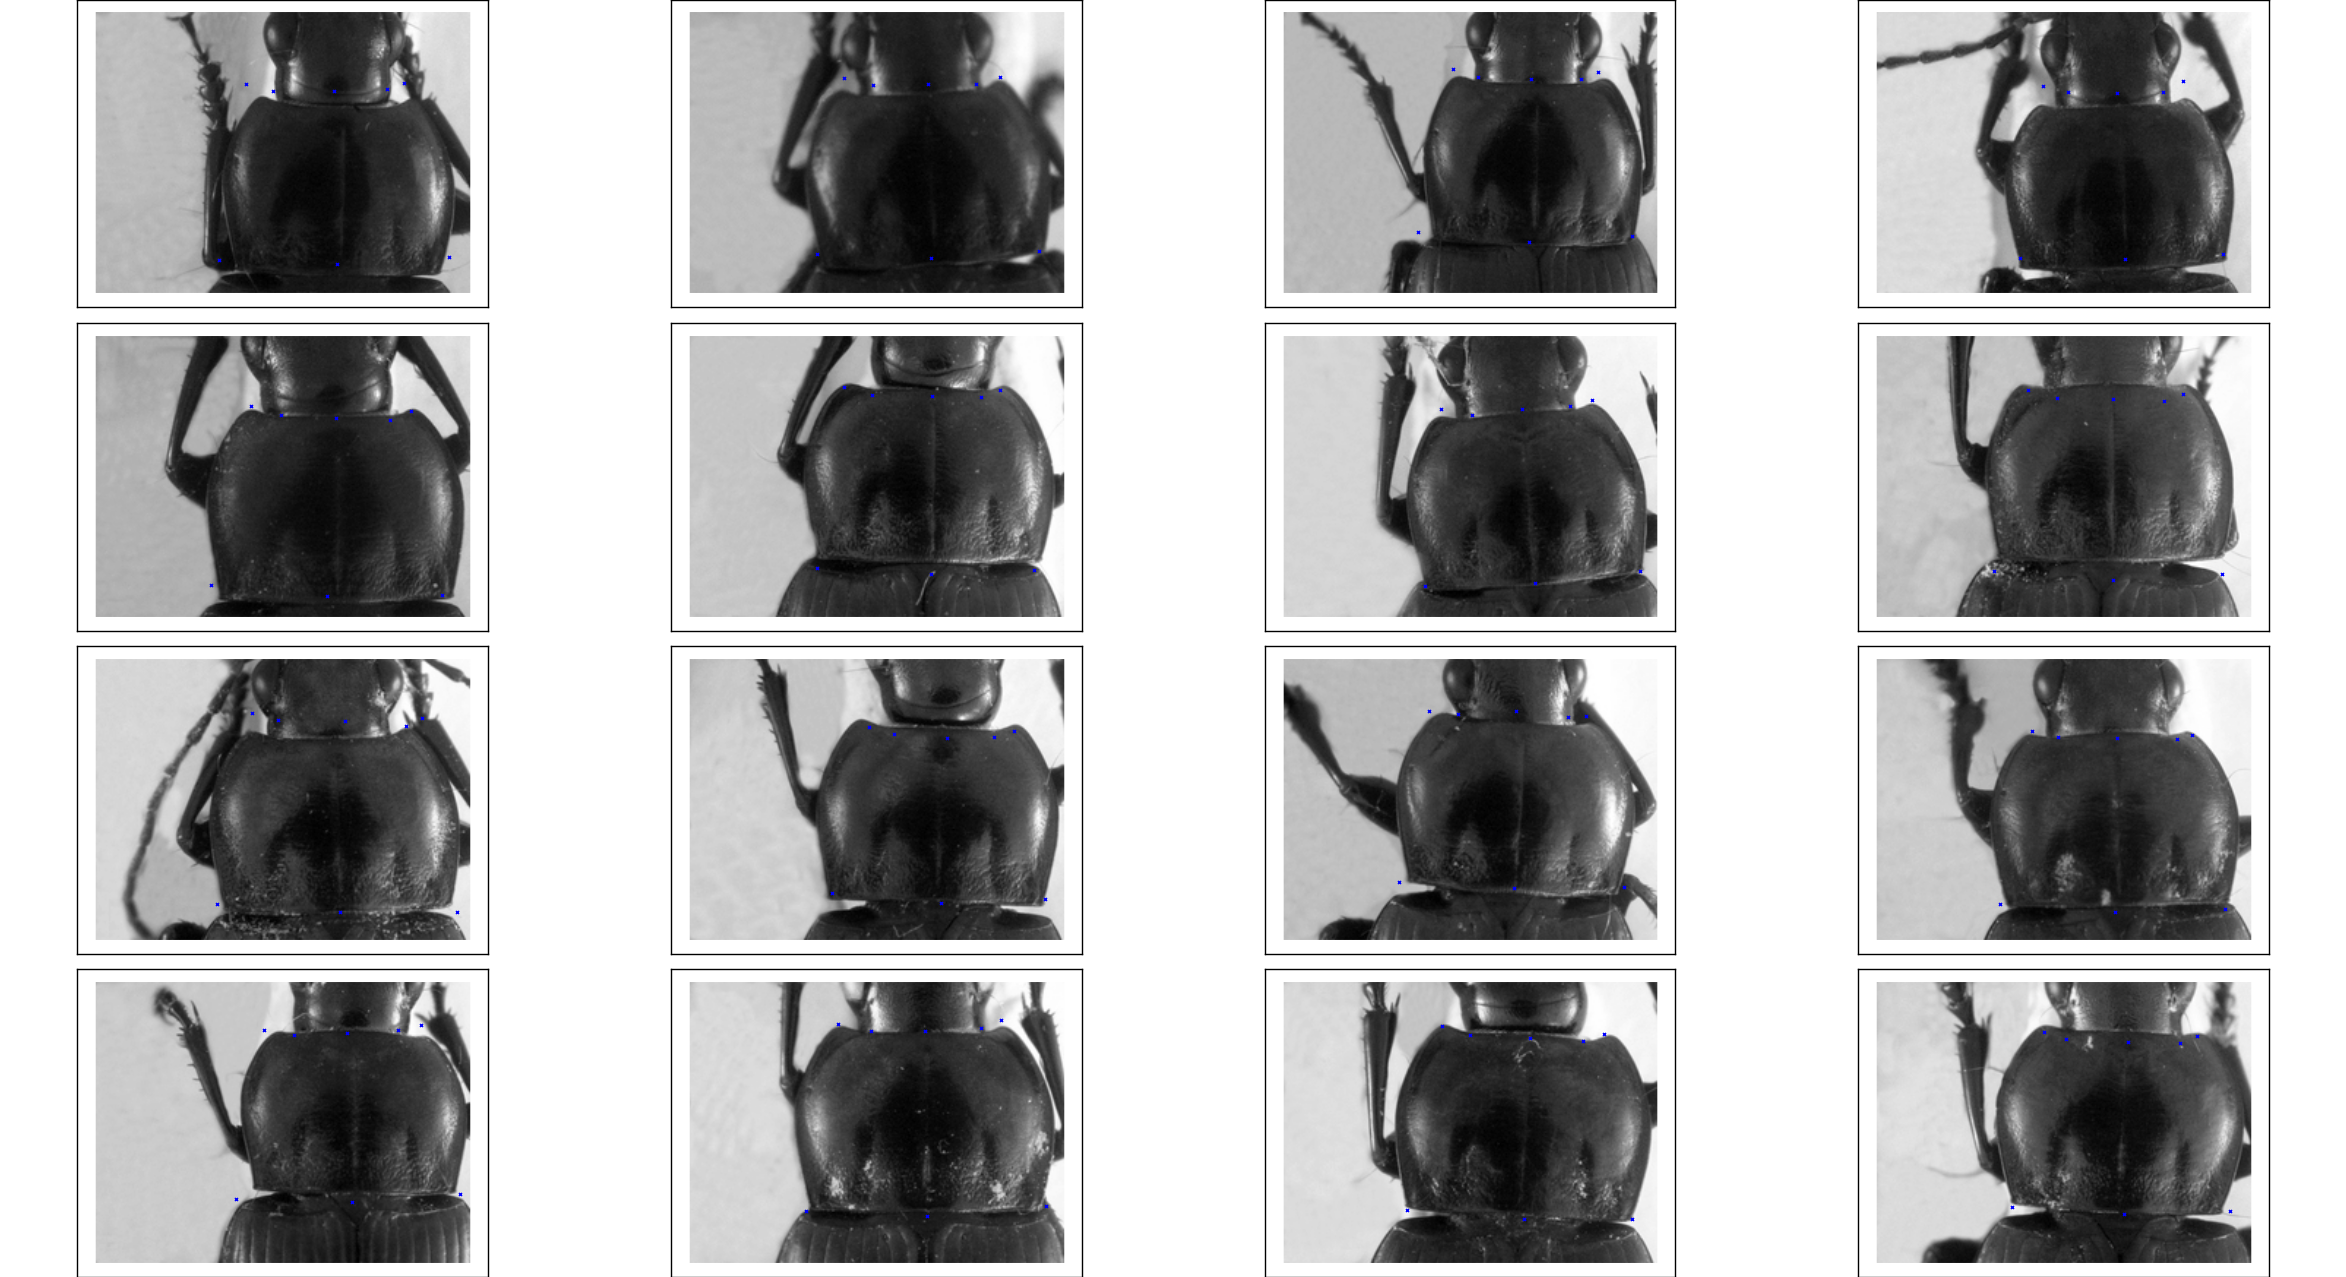
\includegraphics[scale=0.2]{images/figure_1_cnn3_5000_v13}
	\caption{The prediction landmarks on 16-pronotum images}
	\label{cnn3t}
\end{figure}~\\[2cm]
%\begin{figure}[h!]
%	\centering
%	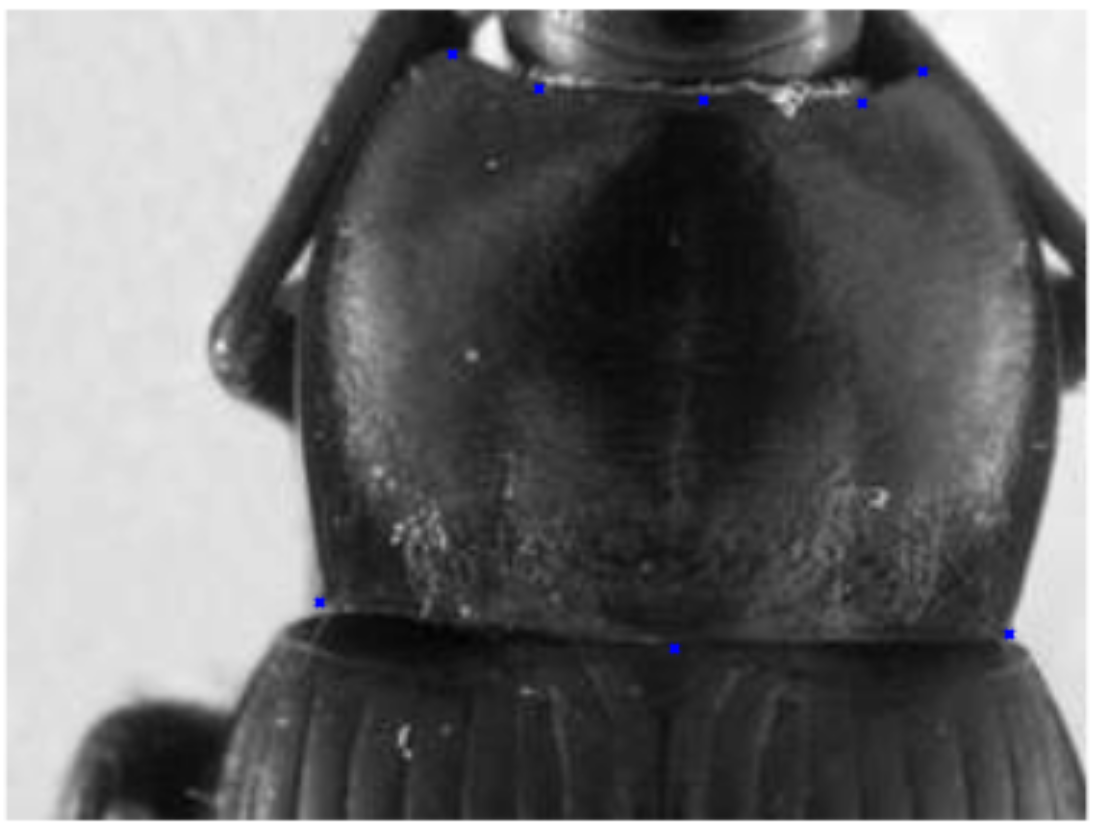
\includegraphics[scale=0.25]{images/plandmark}
%	\caption{The prediction landmarks on a pronotum}
%	\label{cnn3t1}
%\end{figure}
The network in model 3 is applied to predict the landmarks on tete and elytre with some modifications such as: the output at the last of full connected layer. The data that used to train and test are chosen by applying rule\_3. Table.\ref{tete},\ref{elytre} shown the statistic on the test set of tete and elytre by different correlation coefficient methods:
\begin{table}[h!]
	\centering
	\begin{tabular}{l c c}
		Method & x correlation & y correlation \\ \hline
		Pearson & $0.99082758$ & $0.988833$ \\ \hline
		Spearman & $0.9868292$ & $0.989447$ \\ \hline
		Kendall & $0.905933$ & $0.9130359$ \\ \hline
	\end{tabular}
	\caption{The correlation between manual and predicted landmarks on tete images}
	\label{tete}
\end{table}
\begin{table}[h!]
	\centering
	\begin{tabular}{l c c}
		Method & x correlation & y correlation \\ \hline
		Pearson & $0.984969$ & $0.9976646$ \\ \hline
		Spearman & $0.9840307$ & $0.966091$ \\ \hline
		Kendall & $0.8996806$ & $0.846849$ \\ \hline
	\end{tabular}
	\caption{The correlation between manual and predicted landmarks on elytre images}
	\label{elytre}
\end{table}~\\
From the result of Table \ref{losschoosedata}, the dataset which was chosen by rule\_3 is used to continue the experiments. To improve the results, we have modified the rule to pre-process the input data: the target (coordinates of manual landmarks) is normalized into the range of $[-1,1]$, instead of $[0,256]$ for x-coordinate and $[0,192]$ for y-coordinate. Additional, the \textit{learning rate} of the network has been changed to increase the speed of training process.

After changing, the result that we obtain as we expect: training loss and validation loss have decreased significantly(training loss: \textbf{0.00002}, validation loss: \textbf{0.00012}). Thus, the landmarks coordinates have been normalized into $[-1,1]$, so, to calculate the MSE error, we will take the square error and multiply by scale ratio again: the error is arround $1.4$(validation loss). Fig.\ref{tvlscaletarget} shows the losses during training and validation. We can see that overfitting have appeared during the train and validation processes.
\begin{figure}[h!]
	\centering
	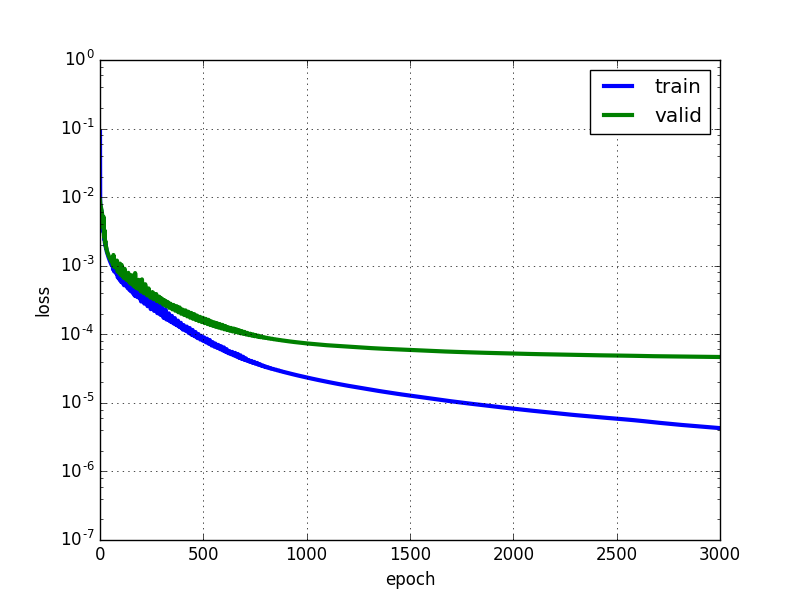
\includegraphics[scale=0.5]{images/figure_1_cnn3_3000_v13_loss_change2}
	\caption{The training and validation loss when normalize the landmarks coordinates}
	\label{tvlscaletarget}
\end{figure}~\\
To prevent the overfitting on the network, we have modified both data and model: on data side, we have changed the \textit{split} ratio to get more samples for validation set($40\%$ instead of $20\%$ of number of samples); on model side, the number of units in the last two hidden layers (full-connected layer) are increased from 500 to 1000. Besides, four dropout layers have been added into the network. They have been located following the pooling layers and the first full-connected layer. The dropout ratios are $0.1$, $0.2$, $0.3$ and $0.5$ (Fig.\ref{model3dropout}).
\begin{figure}[h!]
	\centering
	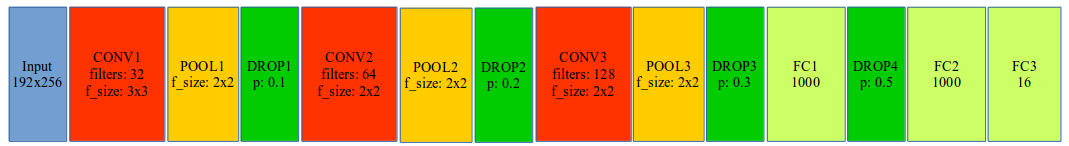
\includegraphics[scale=0.35]{images/model3_dropout}
	\caption{The proposed model with dropout layers}
	\label{model3dropout}
\end{figure}~\\
Fig.\ref{tvldropout} shows the losses after the model have been modified. The overfitting problem is solved but the losses are stability from $2000^{th}$ until the end(we need more data). Table.\ref{coffdropout} shows the correlation coefficient of new model. Clearly that, the result have been improved a little bit when we compare with the last result. 
\begin{figure}[h!]
	\centering
	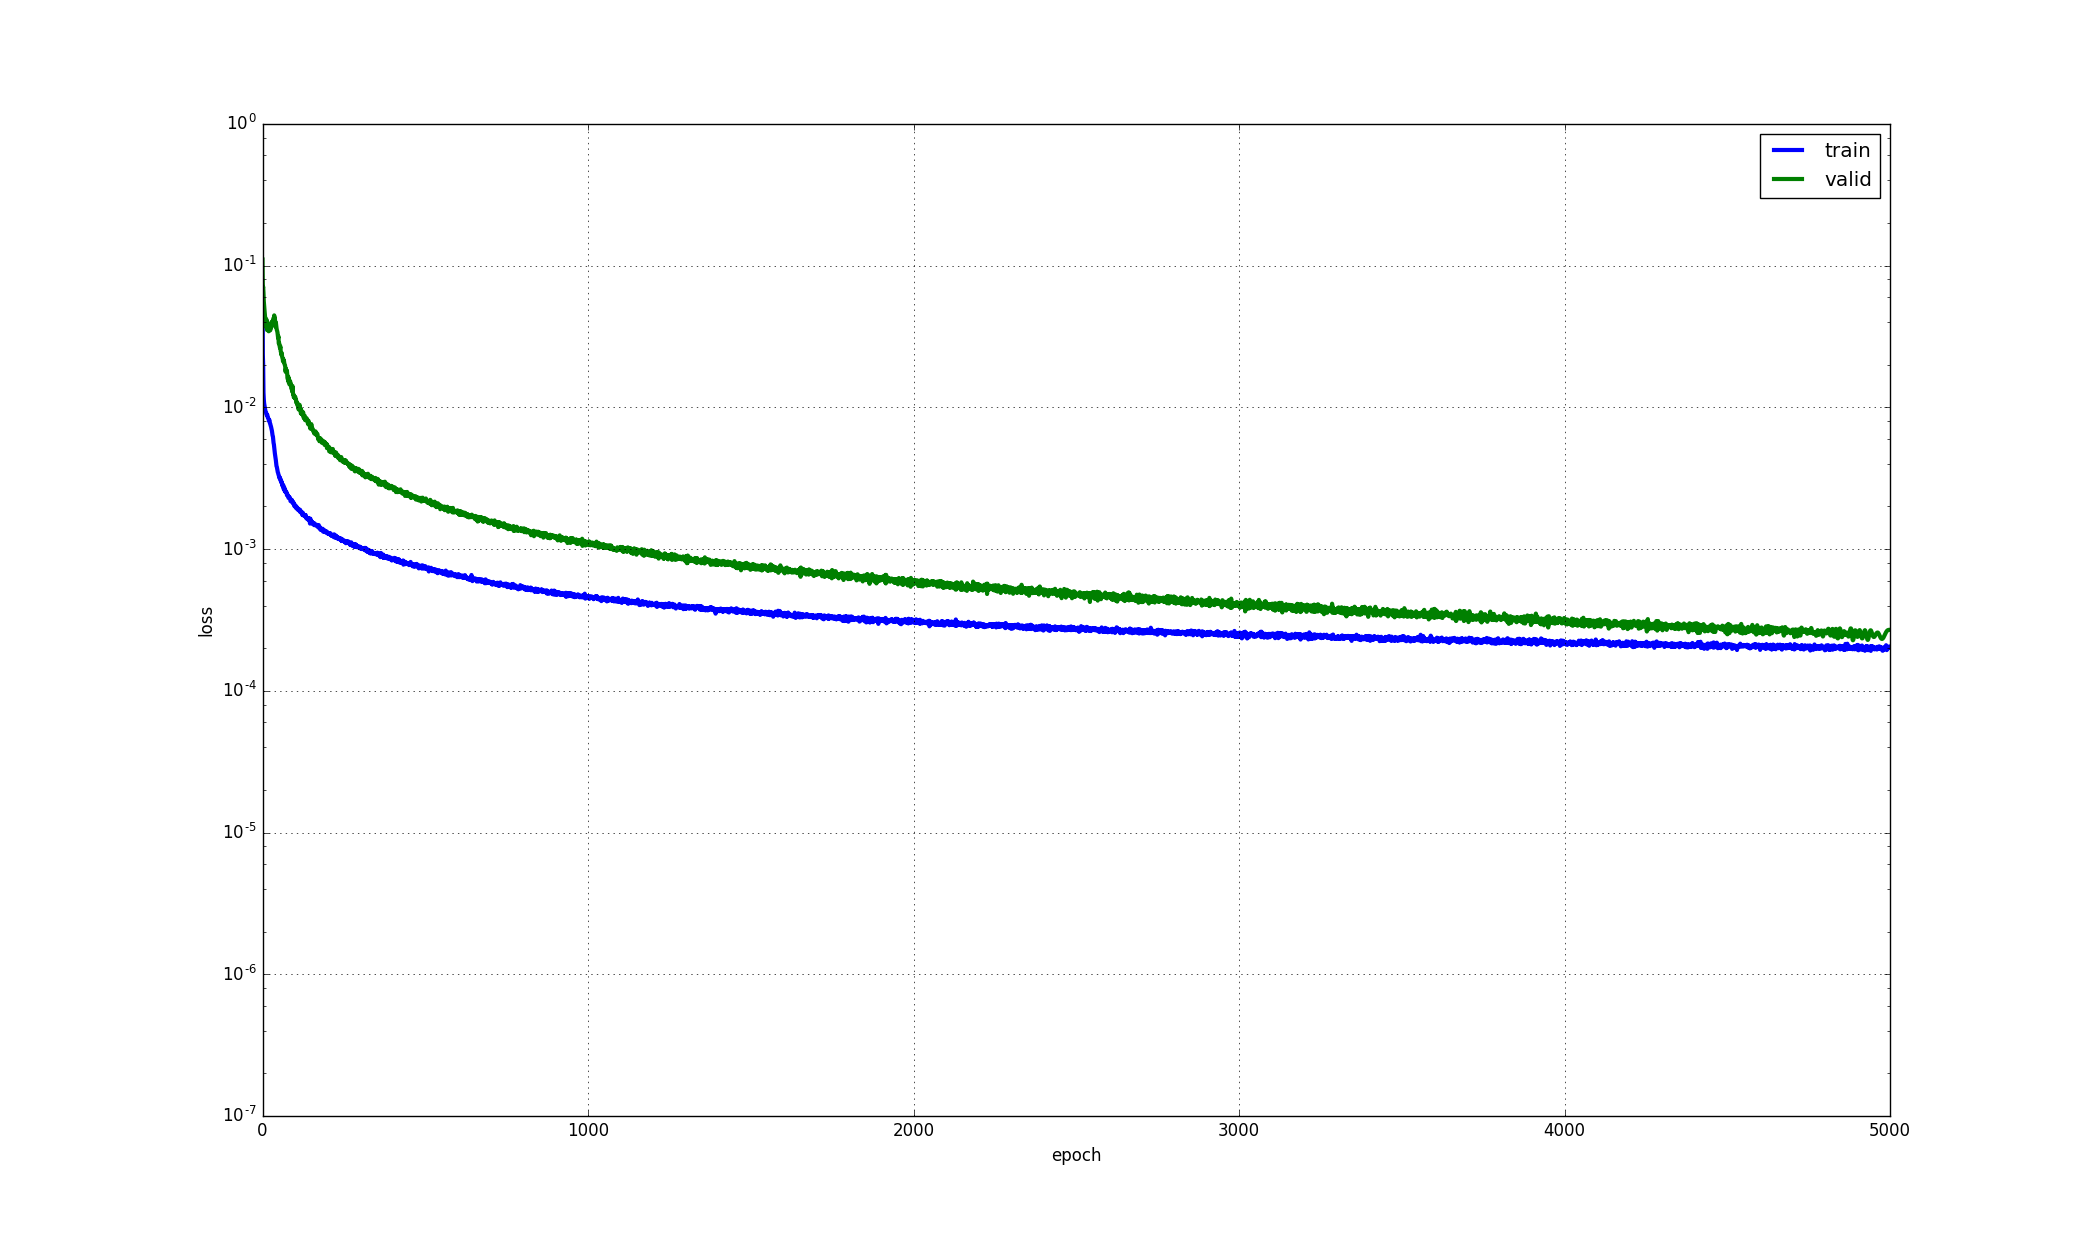
\includegraphics[scale=0.2]{images/figure_1_cnn3_3000_v13_loss_change3_dropout_increase_2}
	\caption{The training and validation loss with dropout layers}
	\label{tvldropout}
\end{figure}~\\
\begin{table}[h!]
	\centering
	\begin{tabular}{l c c}
		Method & x correlation & y correlation \\ \hline
		Pearson & $0.9970585$ & $0.9978605$ \\ \hline
		Spearman & $0.9942475$ & $0.9859642$ \\ \hline
		Kendall & $0.9430501$ & $0.9067739$ \\ \hline
	\end{tabular}
	\caption{The correlation between manual and predicted landmarks on pronotum images with new model}
	\label{coffdropout}
\end{table}
\section{Conclusions}
In this studied, two methods that used to predict the landmarks on 2D gray-scale images are studied. For each case, the model is suitable with different dataset but the results are still not good when we change the data (pronotum). Besides, we proposed a network to learn and detect the landmark positions on pronotum. The accuracy of the model is greater than $98 \%$. The results are evaluated on 3 datasets: pronotum, tete and elytre. From the correlation coefficients of each dataset shows that if we consider on the statistic side, the coefficients are enough good to precise. But when we see the real position on each image, that is not good as we expect. It means the model is not really suitable for the problem and we need to improve the model.
\fi